%======================================================================
\chapter{The Riemann Problem and Riemann Solvers} \label{chap:riemann}
%======================================================================


%====================================================================
\section{The Riemann Problem and Solution Strategy}
%====================================================================

At the heart of finite volume fluid dynamics is the solution to a specific initial value problem
(IVP) called the ``Riemann problem'', as we will see shortly. First, let us define the Riemann
problem: For a hyperbolic system of conservation laws of the form

\begin{align}
	\DELDT{\U} + \DELDX{\F(\U)} = 0
\end{align}

the Riemann problem is defined as

\begin{align}
	\U(x, t=0) =
		\begin{cases}
			\U_L & \text{ if } x < 0\\
			\U_R & \text{ if } x > 0\\
		\end{cases}
\end{align}

which is shown in Figure~\ref{fig:riemann-problem}.

\begin{figure}[H]
\centering
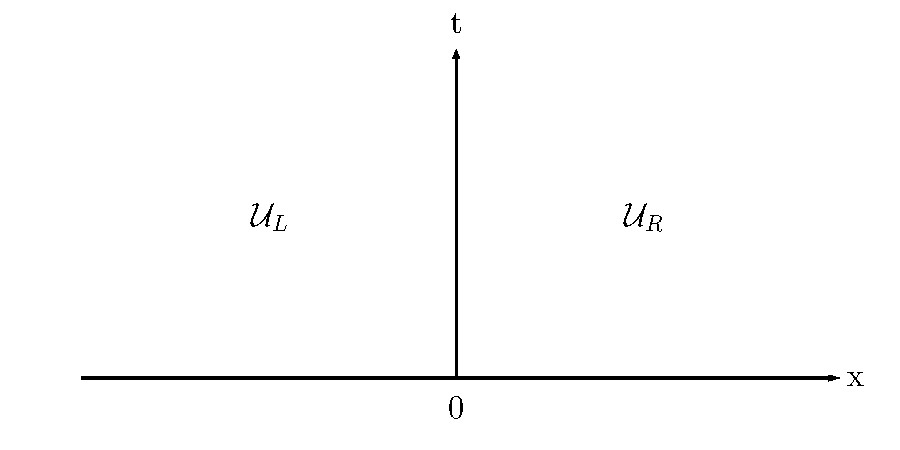
\includegraphics[width=.6\linewidth]{./figures/FV/riemann_problem.pdf}%
\caption{
    The Riemann Initial Value Problem (IVP) in 1D. Two constant initial states, $\U_L$ and $\U_R$,
are initially separated at $x = 0$.
}
\label{fig:riemann-problem}
\end{figure}


In finite volume methods, the fluid (or rather, the conserved quantities) will be discretized
in space by splitting the entire volume into a number of cells (sub-volumes of finite size), each
covering a small fraction of the total volume. Each cell will also keep track of the states $\U$
within their own volume individually. The Riemann problem and the solution thereof enters the game
once we look at what the situation between two adjacent cells is: If we call one of the two adjacent
cells ``the left one'' and the other ``the right one'', then we have \emph{exactly} the Riemann
problem again: Setting $x = 0$ at the interface between two cells, then the state of the left cell
constitutes $\U_L$, while the state of the right cell provides $\U_R$ for the Riemann problem. So in
order to evolve the simulation in time, we need the solution of this Riemann problem in time. In
this chapter, the solution strategies for the Riemann problem are discussed. It begins with the
simple case of the linear advection equation with constant coefficients (eq.
\ref{eq:linear-advection-1D-const-coeff}), and builds up over linear hyperbolic systems all the way
to hyperbolic conservation laws. Later, in Chapter~\ref{chap:godunov}, we will make use of the
Riemann solvers introduced in this Chapter to obtain a numerical method to evolve the Euler
equations for arbitrary initial conditions over any desired interval of time.













%---------------------------------------------------------------------------------------------
\subsection{The Riemann Problem For The Linear Advection Equation With Constant Coefficients}
%---------------------------------------------------------------------------------------------


The solution to the Riemann problem for the linear advection equation with constant coefficients
(eq. \ref{eq:linear-advection-1D-const-coeff}) is somewhat trivial because the equation has an
analytical solution valid for all $t \geq 0$ which is also quite simple:

\begin{align}
    \uc(x, t) = \uc(x - at, 0) \ .
    \label{eq:linear-advection-solution}
\end{align}

This is easily verified by applying the chain rule:

\begin{align}
    \deldt \uc(t) = \DELDX{\uc} \DELDT{(x - at)} = - a \deldx{\uc}
\end{align}

which satisfies eq. \ref{eq:linear-advection-1D-const-coeff}. Effectively, this means that the
solution at a time $t > 0$ is just the initial function $\uc_0(x) = \uc(x, t=0)$ transported (or
rather: \emph{advected}) to the position $x = x_0 + a t$. The solution is illustrated in Fig.
\ref{fig:linear-advection-theory}.


\begin{figure}[H]
    \centering
	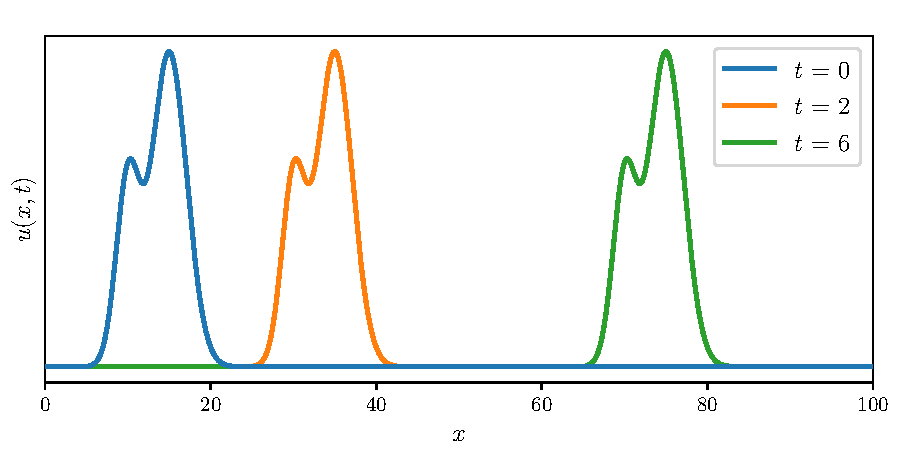
\includegraphics[width=.8\linewidth]{./figures/FV/linear_advection_solution.pdf}%
	\caption[Analytical solution of the linear advection equation with constant coefficients]{
        The analytical solution to the linear advection equation with constant coefficients (eq.
        \ref{eq:linear-advection-1D-const-coeff}) with $a = 10$ in arbitrary units. The initial
        function $\uc_0(x) = \uc(x, t=0)$ is transported (or rather: \emph{advected}) to the
        position $x = x_0 + a t$.
	}
    \label{fig:linear-advection-theory}
\end{figure}


This simple case offers a good opportunity to introduce the notion of \emph{characteristics}, which
will be used in more complex cases as well.  Characteristics may be defined as curves $x = x(t)$
in the $x$-$t$ plane along which the PDE becomes an ordinary differential equation (ODE). Consider
the parametrizaton $x = x(t)$, which makes $\uc = \uc(x(t), t)$. Then the total derivative of $\uc$
w.r.t. time is given by:

\begin{align}
    \DDT{\uc} = \DELDT{\uc} + \DDT{x} \DELDX{\uc} \ .
\end{align}

If now $\DDT{x} = a$, it follows that

\begin{align}
    \DDT{\uc} = \DELDT{\uc} + a \DELDX{\uc} = 0
\end{align}

where the second equality follows from the definition of the linear advection equation. The more
interesting part of this equation is that it gives $\DDT{\uc} = 0$ along the curve $x = x(t)$: it
means that along the characteristic curve which satisfies $\DDT{x} = a$, $\uc$ is constant. On the
$x - t$ plane, $a$ determines the slope of the characteristic. For constant coefficients $a$, all
characteristics are parallel. To determine the solution at some $(x, t > 0)$, all we need to do is
follow the characteristic that goes through that point back to $t = 0$.

Coming back to the Riemann problem for linear advection equations with constant coefficients, it
can explicitly be written as:

\begin{align}
    & \deldt \uc + a \deldx \uc = 0 &&\\
    & \uc(x, 0) = \uc_0 (x) = \begin{cases}
                             \uc_L & \text{ if } x < 0 \\
                             \uc_R & \text{ if } x > 0
                            \end{cases} &&
\end{align}


This IVP is illustrated in Fig.~\ref{fig:riemann-linear-advection}. Using the general solution
\ref{eq:linear-advection-solution}, it follows that the solution for the Riemann problem is given
by:

\begin{align}
    \uc(x, t) = \uc_0(x - at) = \begin{cases}
                                    \uc_L & \text{ if } x - at < 0 \\
                                    \uc_R & \text{ if } x - at > 0
                                \end{cases}
\end{align}

which is illustrated in Fig. \ref{fig:riemann-linear-advection}. In other words: The two initial
states $\uc_L$ and $\uc_R$ will be separated on the $x - t$ plane by the characteristic that
satisfies $\DDT{x} = a$.


\begin{figure}[H]
    \centering
	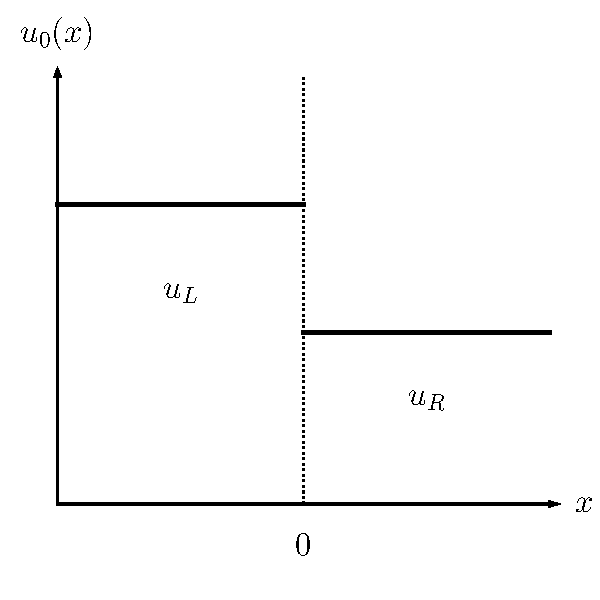
\includegraphics[width=.4\linewidth]{./figures/FV/riemann_problem_linear_advection.pdf}%
	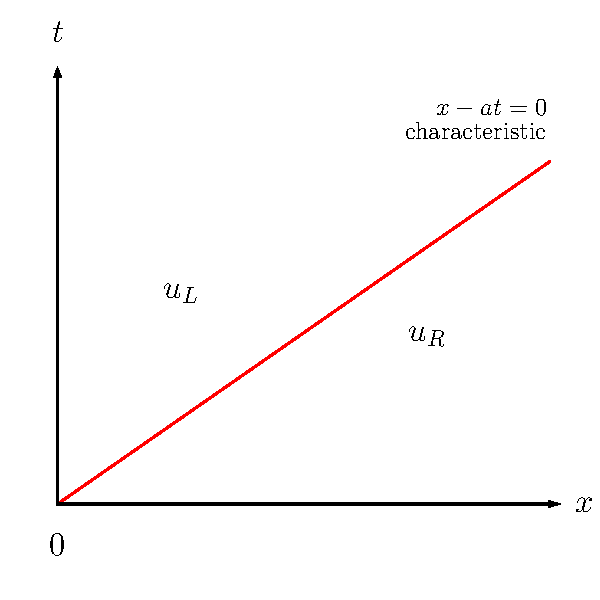
\includegraphics[width=.4\linewidth]{./figures/FV/riemann_solution_linear_advection.pdf}%
	\caption[Riemann problem and solution for the linear advection equation with constant
coefficients]{
    Left: The initial Riemann problem for the linear advection equation with constant
coefficients. Right: The solution to the Riemann problem. For $t > 0$, the two initial states
$\uc_L$ and $\uc_R$ will be separated by the $x - at = 0$ characteristic.
	}
    \label{fig:riemann-linear-advection}
\end{figure}













%---------------------------------------------------------------------
\subsection{The Riemann Problem For Linear Hyperbolic Systems}
%---------------------------------------------------------------------


Let's now extend the analysis to linear hyperbolic systems, i.e. sets of $m$ hyperbolic PDEs of the
form

\begin{align}
    \deldt \U + \mathcal{A} \deldx \U = 0 \label{eq:linear-hyperbolic-system}
\end{align}

with $\mathcal{A} = \CONST$
By definition of a hyperbolic system, $\mathcal{A}$ has $m$ real
eigenvalues $\lambda_i$ and $m$ linearly independent eigenvectors $\mathbf{K}_i$. This allows
$\mathcal{A}$ to be expressed in diagonalized form, i.e. in terms of a diagonal matrix $\Lambda$
and the matrix $\mathcal{K}$:

\begin{align}
 \mathcal{A} = \mathcal{K} \ \Lambda \ \mathcal{K}^{-1} \quad \text{or} \quad
 \Lambda = \mathcal{K}^{-1} \mathcal{A} \mathcal{K}
\end{align}

where $\Lambda$ is a diagonal matrix whose diagonal elements are the eigenvalues $\lambda_i$, and
$\mathcal{K}$ is the matrix whose columns $\mathcal{K}^{(i)}$ are the right eigenvectors
$\mathbf{K}_i$ of $\mathcal{A}$ corresponding to the eigenvalues $\lambda_i$. To make use of
$\mathcal{K}$, we first note that since $\mathcal{A}$ is constant, $\mathcal{K}$ must be too, and
therefore $\deldt \mathcal{K} = \deldx \mathcal{K} = 0$.

By defining

\begin{align}
 \W = \mathcal{K}^{-1} \U \quad \text{ or } \quad \U = \mathcal{K} \W
\end{align}

we can write eq.~\ref{eq:linear-hyperbolic-system} as

\begin{align}
  \mathcal{K} \deldt \W + \mathcal{A} \mathcal{K} \deldx \W = 0
\end{align}

Applying $\mathcal{K}^{-1}$ from the left on the entire equation gives us a neat result:


\begin{align}
  \mathcal{K}^{-1} \mathcal{K} \deldt \W + \mathcal{K}^{-1} \mathcal{A} \mathcal{K} \deldx \W  =
  \deldt \W + \Lambda \deldx \W = 0 \label{eq:canonical-form}
\end{align}

Eq.~\ref{eq:canonical-form} is called the canonical or characteristic form of the system. In this
form, the system is decoupled: Recall that $\Lambda$ is a diagonal matrix, and hence the $i$-th PDE
of the system is given by

\begin{align}
    \deldt \wc_i + \lambda_i \deldx \wc_i = 0 \quad \quad i = 1, \dots, m
\end{align}

and in this form is identical to the linear advection equation with constant coefficients, for
which we have a solution. The characteristic speed is now $\lambda_i$, and the characteristic curves
need to satisfy $\DDT{x} = \lambda_i$. So we have effectively transformed a system of $m$ coupled
PDEs into a system of $m$ independent linear advection equation with constant coefficients.

In order to obtain the solution in terms of the original variables $\U$, the transformation

\begin{align}
    \U(x,t) = \mathcal{K} \W(x,t)
\end{align}

or component-wise

\begin{align}
    \U_j(x,t) = \sum_i^m \wc_i(x,t) \mathcal{K}_{ij}
\end{align}

must be calculated. The solution for $t > 0$ is then given by applying the characteristic solution:


\begin{align}
    \U_j(x,t) = \sum_i^m \wc_i(x,t) \mathcal{K}_{ij} = \sum_i^m \wc_i(x - \lambda_i t,t=0)
\mathcal{K}_{ij}
\end{align}

So given a point $(x, t)$ on the $x-t$ plane, the solution $\U(x,t)$ at this point depends again
only on the initial data. However, contrary to the linear advection equation with constant
coefficients, this time we were dealing with a system of $m$ equations, and so it is natural that
the solution at a point $(x, t)$ depends on $m$ points of the initial data, or more precisely the
points $x_0^{(i)} = x - \lambda_i t$. These are the intersections of the characteristics with
velocities $\lambda_i$ with the $x$-axis. The solution for $\U(x,t)$ can be seen as the
superposition of $m$ waves, each of which is advected independently and without change in shape due
to the constraint that $\mathcal{A} = \CONST$
The $i$-th wave has the shape $\wc_i(t=0)
\mathbf{K}^{(i)}$ and speed $\lambda_i$.

Let us now formulate the solution for the Riemann problem for linear hyperbolic systems, which is
given by:

\begin{align}
    & \deldt \U + \mathcal{A} \deldx \U = 0 && \\
    & \U(x, 0) = \U^{(0)} (x) = \begin{cases}
                               \U_L & \text{ if } x < 0 \\
                               \U_R & \text{ if } x > 0
                              \end{cases} &&
\end{align}



\begin{figure}[H]
    \centering

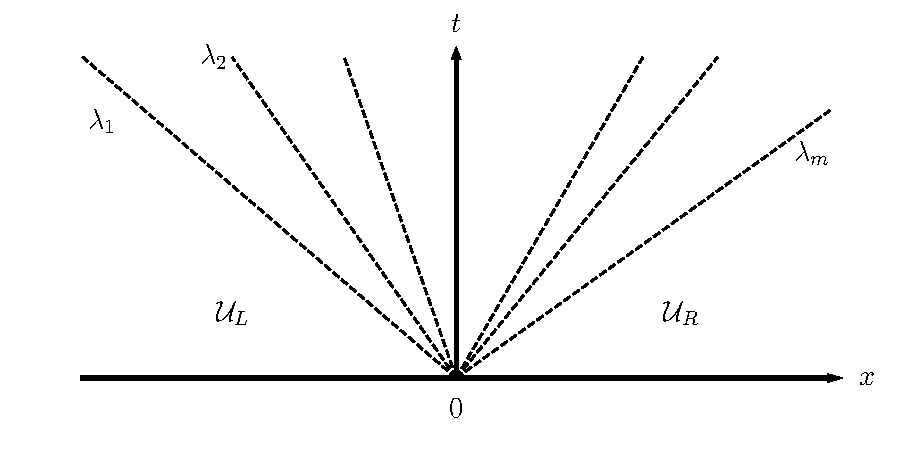
\includegraphics[width=.7\linewidth]{./figures/FV/riemann_solution_linear_hyperbolic_systems.pdf}%
	\caption[Structure of the solution of the Riemann problem for linear hyperbolic systems]{
	The structure of the solution of the Riemann problem for linear hyperbolic systems. For each of
the $m$ eigenvalues $\lambda_i$ of the problem a characteristic with speed $\lambda_i$ will form a
jump discontinuity between two states.}
    \label{fig:riemann-linear-hyperbolic-system}
\end{figure}


If we assume that the system is strictly hyperbolic, we can index the eigenvalues
$\lambda_i$ such that $\lambda_1 < \lambda_2 < \ldots < \lambda_m$. The structure of the solution
consists of $m$ waves emanating from the origin, one for each eigenvalue $\lambda_i$ (see
Fig.~\ref{fig:riemann-linear-hyperbolic-system}). Waves for which $\lambda_i > 0$ will advect the
component $\wc_{i,L} = \oldsum_j \mathcal{K}_{ij}^{-1}\U_{L,j}$ into regions where $x > 0$ and
where the initial state was $\U_R$, while waves for which $\lambda_i < 0$ will advect the component
$\wc_{i,R} = \oldsum_j \mathcal{K}_{ij}^{-1}\U_{R,j}$ into regions where $x < 0$ and where the
initial state was $\U_L$.
To find a precise expression for the general solution, we can make use of the fact that the
eigenvectors $\mathbf{K}^{(i)}$ are linearly independent, meaning that we can express any state $\U
= \oldsum_i^m \gamma_i \mathbf{K}^{(i)}$ as linear combinations of the eigenvectors. That allows us
to define

\begin{align}
  \U_L = \sum_i^m \alpha_i \mathbf{K}^{(i)} \quad \text{ and } \quad
  \U_R = \sum_i^m \beta_i \mathbf{K}^{(i)}
\end{align}

From the general solution, we know that $\U(x, t) = \oldsum_i \wc_i \mathbf{K}^{(i)}$ with

\begin{align}
    \wc_i(x, t) = \wc_i(x - \lambda_i t, 0) = \begin{cases}
                                               \alpha_i & \text{ if } x - \lambda_i t < 0 \\
                                               \beta_i & \text{ if } x - \lambda_i t > 0 \\
                                              \end{cases}
\end{align}

Alternatively, it can be rewritten by defining the index $I$ for any given point $(x, t)$ such that
the eigenvalues $\lambda_I \leq \frac{x}{t} < \lambda_{I+1}$, i.e. $x - \lambda_i t > 0\ \forall i
\leq I$. Then the solution is given by

\begin{align}
    \U(x, t) = \sum_{i = I+1}^m \alpha_i \mathbf{K}^{(i)} + \sum_{i=1}^I \beta_i \mathbf{K}^{(i)}
\end{align}
















%---------------------------------------------------------------------
\subsection{The Riemann Problem For Hyperbolic Conservation Laws}
%---------------------------------------------------------------------

Finally, let's look into the Riemann problem for hyperbolic conservation laws, whose solution we
will require to construct numerical methods to solve fluid dynamics and radiative transfer. For
simplicity, let's consider only a single equation instead of an entire system of equations to start
with, i.e.

\begin{align}
    \deldt \uc + \deldx \fc(\uc) = 0
\end{align}

which can also be written in the form

\begin{align}
    \deldt \uc + \alpha(\uc) \deldx \uc = 0
\end{align}

where $\alpha(\uc) = \frac{\partial \fc}{\partial \uc}$ is not constant any longer, but a function
of $\uc$. We can once again apply the method of characteristics and set $\DDT{x} = \alpha(\uc)$,
giving us

\begin{align}
    \DDT{\uc} = \deldt \uc + \alpha(\uc) \deldx \uc = 0
\end{align}

Just like in the previous cases, $\uc$ is constant along these characteristics. Even though the
characteristic speeds $\alpha(\uc)$ depend on the state $\uc$, given that $\uc$ is constant along
the characteristic, characteristic speeds themselves are constant as well. Therefore, once again
the characteristic curves are straight lines. However, they aren't identical over all $x$ any more,
and the translation distorts the the initial function as time evolves. This is a distinguishing
feature of non-linear problems. To illustrate why and how the complications arise, let's consider a
concrete example of a conservation law: The (inviscid) Burgers equation, given by:

\begin{align}
    \deldx \uc + \uc \deldx \uc = 0  \label{eq:inviscid-burgers}
\end{align}


which has characteristic speeds $\alpha(\uc) = \uc$. The Burgers equation can be obtained from the
momentum equation of the Euler equations and the additional assumption that the fluid density (and
therefore also pressure) variations are negligible. Figure~\ref{fig:burgers-characteristics} shows
an example of some initial state $\uc(x, t=0)$ on the left side, and the corresponding
characteristic lines on the right. The complications are evident: The characteristics can now fan
out and diverge in so-called ``expansive regions'' as is the case around $x \sim 20$ in
Figure~\ref{fig:burgers-characteristics}. Or they can get narrower and steeper as time evolves in
so-called ``compressive regions'', as is happens around $x \sim 50$ and $x \sim 90$ in
Figure~\ref{fig:burgers-characteristics}. This steepening, called ``wave steepening'', results in
the characteristics eventually intersecting, at which point our solution breaks down: there is no
single-valued solution any longer. The initial $\uc$ should be constant along their
characteristics, but that cannot be the case at the point of an intersection, where they are
supposed two have more than one value simultaneously. And we know  for a fact that the two
intersecting characteristics must stem from two different initial values $\uc$, because the slope of
the characteristics is $\alpha(\uc)$. In order for characteristics to intersect, the slopes can't be
equal, otherwise the characteristics would be parallel and never intersect.

In general, expansive regions can be found in regions where $\deldx \alpha(\uc)
> 0$, while compressive regions are regions where initially $\deldx \alpha(\uc) > 0$. In regions of
constant characteristic speeds $\deldx \alpha(\uc) = 0$, the solution is the same as for linear
hyperbolic systems.




\begin{figure}[H]
    \centering
    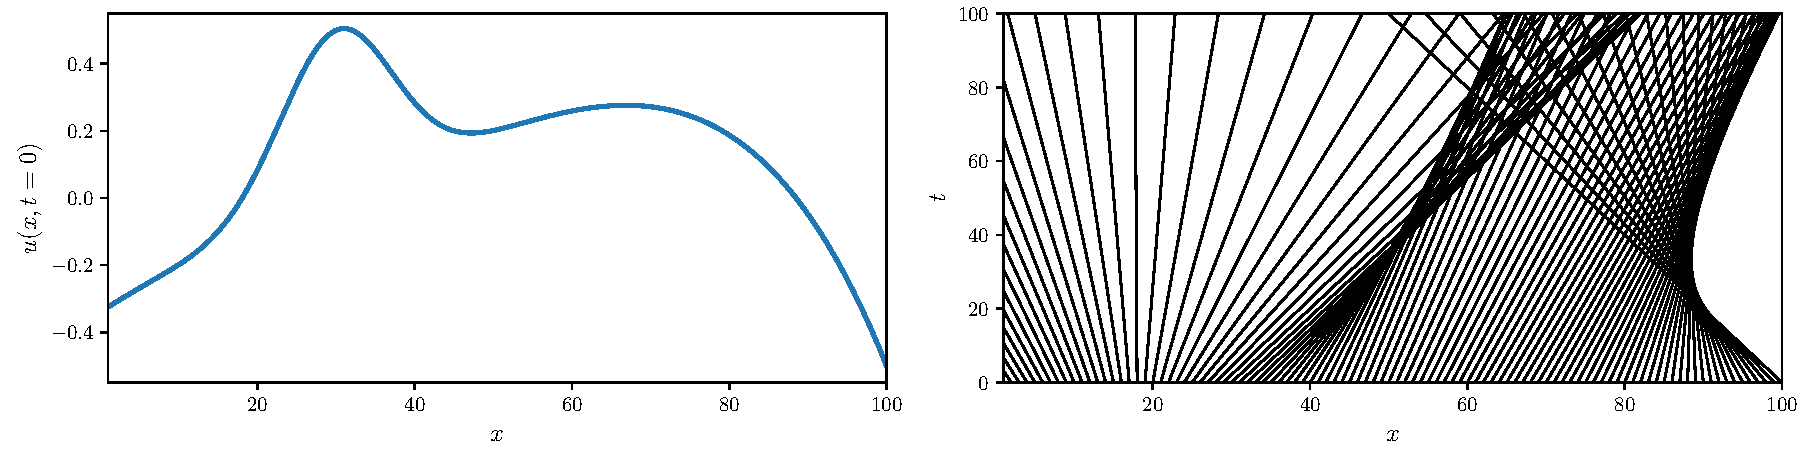
\includegraphics[width=\linewidth]{./figures/FV/burgers_characteristics.pdf}%
    \caption[Characteristics for the Burgers equation]{
    Left: Some initial conditions $\uc_0(x, t=0)$ for the Burgers'
equation~(\ref{eq:inviscid-burgers}). Right: The corresponding characteristics that satisfy
$\DDT{x} = \uc$. All units are arbitrary.
}
    \label{fig:burgers-characteristics}
\end{figure}


There are two approaches to deal with this occurrence. One option is to modify the equation (and
the physical system) that is being solved to not allow wave steepening, e.g. by introducing a
``viscous'' or diffusive term that is proportional to the second derivative of $\uc$ w.r.t. $x$.
This term will then have the exact opposite, wave-easing, effect: as the wave steepens, $\deldx
\uc$ increases, and so does $\frac{\del^2}{\del x^2} \uc$, having a proportionally stronger effect
in the opposite direction of the steepening, and counteracting it in this manner.

The other alternative is to stick to the inviscid equation, but to allow for discontinuous
solutions, i.e. shocks, to be formed as a process of increasing compression. The states left and
right of the shock wave are then determined ``as usual'' by the method of characteristics, while
the shock wave itself is modeled as a jump discontinuity at the points where the characteristics
intersect. To illustrate this approach, the shape of the solution for a Riemann problem for the
Burgers equation is depicted in Fig.~\ref{fig:burgers-riemann-shock}.

\begin{figure}[H]
    \centering
    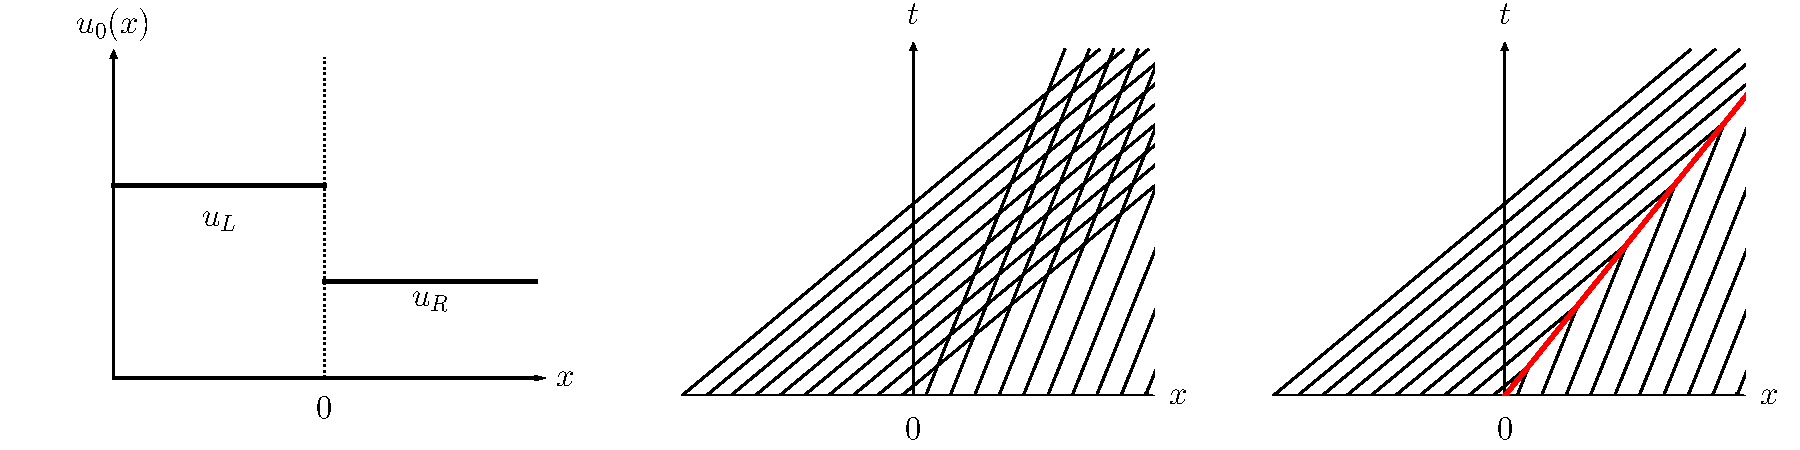
\includegraphics[width=\linewidth]{./figures/FV/burgers_riemann_shock.pdf}%
    \caption[Characteristics and shock wave for the Riemann problem of Burgers equation]{
    Left: A shock generating Riemann problem initial conditions $\uc_0(x)$ for the inviscid Burgers
equation~(\ref{eq:inviscid-burgers}). Middle: The corresponding characteristics. Right: The
resulting shock wave (in red), which is a jump discontinuity.
}
    \label{fig:burgers-riemann-shock}
\end{figure}

Modeling a shock wave as a jump discontinuity is all good and well, but an important question
remains: What is the velocity of the shock wave going to be? To answer this question we need to
resort to using the integral form of conservation laws, so we can deal with the discontinuity in an
appropriate manner. The integral form is given by integrating the entire conservation law equation
(eq.~\ref{eq:conservation-law-1D-introduction}) over both a space interval $x \in [x_0, x_1]$ and
time interval $t \in [t_0, t_1]$:

\begin{align}
    \int\limits_{x_0}^{x_1} \int\limits_{t_0}^{t_1} \left[\deldt \U + \deldx \F \right] \de x \de t
= 0 \ .
\end{align}

The right hand side equality is trivially satisfied by virtue of the integrand,
eq.~\ref{eq:conservation-law-1D-introduction}, always satisfying it. We can immediately deal
away with the partial derivatives:

\begin{align}
    \int\limits_{x_0}^{x_1} \int\limits_{t_0}^{t_1} \left[\deldt \U + \deldx \F \right] \de x \de t
=
    \int\limits_{x_0}^{x_1} \left[ \U(x, t_1) - \U(x, t_0) \right] \de x +
    \int\limits_{t_0}^{t_1} \left[ \F(x_1, t) - \F(x_0, t) \right] \de t \ .
    \label{eq:rankine-hugeniot-integral}
\end{align}

To determine the shock speed $S$, consider a solution $\U(x,t)$ such that $\U(x,t)$ and $\F(x,t)$
are continuous everywhere except on a line $S = S(t)$ on the $x-t$ plane. Across this line,
$\U(x,t)$ has a jump discontinuity. Let us refer to states and fluxes ``left'' of $S(t)$, i.e.
where $x < S(t)$, as $\U_L$ and $\F_L$. Similarly, let the states and fluxes to the ``right'', i.e.
where $x > S(t)$, be $\U_R$ and $\F_R$. Furthermore, select two points in space, $x_0$ and $x_1$
with $x_0 < x_1$, and two points in time, $t_0$ and $t_1$ with $t_0 < t_1$, such that both points
$(x_0, t_0)$ and $(x_1, t_1)$ coincide with the shock wave $S(t)$ on the $x-t$ plane, and
consequently the position of the shock can be inferred by $x_1 = x_0 + S (t_1 - t_0)$. This
situation is illustrated in Figure~\ref{fig:rankine-hugeniot}.


\begin{figure}[H]
    \centering
    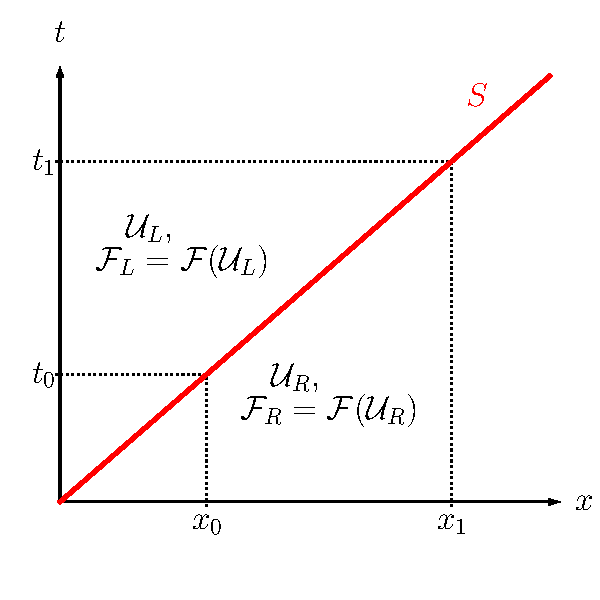
\includegraphics[width=.5\linewidth]{./figures/FV/rankine_hugeniot.pdf}%
    \caption[Setup for the Rankine-Hugeniot conditions]{
Setup to derive the Rankine-Hugeniot conditions with a constant left state $\U_L$ and flux
$\F_L$ and a right state $\U_R$ and corresponding flux $\F_R$, which are separated by a jump
discontinuity which propagates at constant velocity $S$.
}
    \label{fig:rankine-hugeniot}
\end{figure}


If the shock is indeed infinitely thin, the states $\U_{L,R}$ are homogeneous over space, and the
fluxes $\F_{L,R}$ are homogeneous over time, then we can see that

\begin{align}
    \U(t_1, x) = \U_L &&  \U(t_0, x) = \U_R && \forall x \in [x_0, x_1] \\
    \F(t, x_1) = \F_R &&  \F(t, x_0) = \F_L && \forall t \in [t_0, t_1]
\end{align}

using these relations, the integral \ref{eq:rankine-hugeniot-integral} is easily solved:

\begin{align}
    &
    \int\limits_{x_0}^{x_1} \left[ \U(x, t_1) - \U(x, t_0) \right] \de x +
    \int\limits_{t_0}^{t_1} \left[ \F(x_1, t) - \F(x_0, t) \right] \de t = &&\\
%
    &
    \int\limits_{x_0}^{x_1} \U(x, t_1) \de x -
    \int\limits_{x_0}^{x_1} \U(x, t_0) \de x +
    \int\limits_{t_0}^{t_1} \F(x_1, t) \de t -
    \int\limits_{t_0}^{t_1} \F(x_0, t) \de t = &&\\
    &
    \int\limits_{x_0}^{x_1} \U_L \de x -
    \int\limits_{x_0}^{x_1} \U_R \de x +
    \int\limits_{t_0}^{t_1} \F_R \de t -
    \int\limits_{t_0}^{t_1} \F_L \de t = &&\\
    &
    - ( \U_R - \U_L)(x_1 - x_0) + (\F_R - \F_L) (t_1 - t_0) = 0 &&
\end{align}

which finally leads to

\begin{align}
    \F_R - \F_L &= \frac{x_1 - x_0}{t_1 - t_0} \left( \U_R - \U_L \right) \\
                &= S \left( \U_R - \U_L \right) \label{eq:rankine-hugeniot}
\end{align}

Expression~\ref{eq:rankine-hugeniot} is called the Rankine-Hugeniot conditions, which gives us the
shock propagation speed $S$ as well as a relation between states and fluxes across discontinuities.






%------------------------------------------------------------------------------------
\subsubsection{Requirements For Physically Meaningful Shocks and Rarefaction Waves}
%------------------------------------------------------------------------------------

An additional point needs to be made for shocks in order for them to be physical solutions: They
need to arise from compressive regions. Following the sketch in Figure~\ref{fig:rankine-hugeniot},
that translates to the condition that the characteristic speeds $\alpha_L$ and $\alpha_R$ must obey
$\alpha_L > \alpha_R$, i.e. they must converge into the discontinuity. This condition is called
the ``entropy condition''. The inverse case, where $\alpha_L < \alpha_R$ for two states $\U_L$ and
$\U_R$ separated by a jump discontinuity, is mathematically permissible, but physically
nonsensical: In case of these ``rarefaction shocks'' characteristics diverge from the discontinuity.
Given that the characteristics carry information about the state they emanate from, this would mean
that new information must be generated out of nowhere along the discontinuity to be carried. This is
an entropy violating condition, as in the case of gas dynamics, it contradicts the second law of
thermodynamics. The second law of thermodynamics states that the entropy of a system must be
non-decreasing. This is the case for compressive shocks, across which the entropy of a system
increases. Since the entropy at each point can be computed as a function of pressure and density
(see eq.~\ref{eq:entropy}), and it increases for compressive shocks, it follows that for the case
of rarefaction shocks, where the inverse behavior to compressive shocks occurs, the entropy must
decrease. This is an unphysical solution.

Furthermore, the rarefaction shock solution is unstable under small perturbations, in the sense
that small perturbations of the initial data lead to large changes in the solution. To demonstrate
that point, let's modify the initial conditions from a rarefaction generating Riemann problem,
i.e. from two constant states $\uc_L$ and $\uc_R$ with diverging characteristics. Take two points
$x_L$ and $x_R$, which are separated by some distance $\Delta x$. Then let the states with $x < x_L$
be constant and called $\uc_L$, the states with $x > x_R$ be constant and called $\uc_R$, while the
state in the intermediate region $\Delta x$ between them increase linearly between $\uc_L$ and
$\uc_R$, i.e.

\begin{align}
    \uc_0(x) = \begin{cases}
                 \uc_L                                      & \text{ if } x \leq x_L \\
                 \uc_L + (\uc_R - \uc_L)\frac{x - x_L}{x_R - x_L} & \text{ if } x_L < x < x_R \\
                 \uc_R                                      & \text{ if } x \geq x_R   \\
               \end{cases} \label{eq:rarefaction-setup}
\end{align}

\begin{figure}[H]
    \centering
    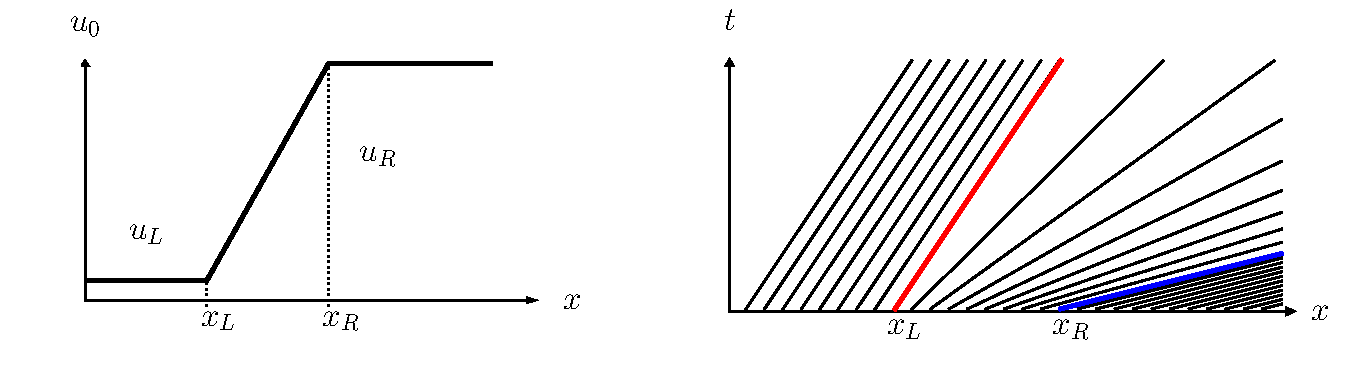
\includegraphics[width=\linewidth]{./figures/FV/rarefaction_characteristics.pdf}%
    \caption[Rarefaction wave characteristics]{
Left: The initial conditions described by eq.~\ref{eq:rarefaction-setup}, in arbitrary units.
Right: The corresponding characteristics. The two outermost characteristics of the intermediate
region $x_L < x < x_R$ are highlighted: The tail of the rarefaction wave is in red, while the head
is in blue.
}
    \label{fig:rarefaction-setup}
\end{figure}

These initial states and the corresponding characteristics (assuming once again the inviscid
Burgers' equation for simplicity) are shown in Fig.~\ref{fig:rarefaction-setup}. Two special
characteristics at the outer edges of the intermediate region can be identified, namely the ones
that overlap with the characteristics of the outer constant regions. Assuming a convex flux, i.e.
$\deldx \alpha(\uc) > 0$  (as is done in Fig.~\ref{fig:rarefaction-setup}), larger values of $\uc$
propagate faster that lower values, hence the characteristics of $\uc_R$ propagate faster than
those of $\uc_L$. The rightmost characteristic of the intermediate region will have the same
propagation speed as the right constant region, i.e. satisfy $x = x_R + \alpha(\uc_R)t$. This wave
is called the \emph{head} of the rarefaction wave, which is marked blue in
Figure~\ref{fig:rarefaction-setup}. Similarly, the leftmost characteristic satisfies $x = x_L +
\alpha(\uc_L) t$, and is called the \emph{tail} of the rarefaction wave, marked in red in
Figure~\ref{fig:rarefaction-setup}. As for all the other characteristics between the head and the
tail, a region called the ``rarefaction fan'', mathematically they pose no new problem. There are
no intersections nor undefined regions there. It's true that they diverge, but every point $(x, t)$
enclosed by the head and the tail characteristics can still be solved by tracing back the
characteristics to the initial time, just as for linear hyperbolic systems. A major difference to
linear systems however remains the fact that the propagation velocities aren't identical across the
intermediate section: The closer we are to the right state $\uc_R$ as seen from the inside of the
fan, the higher $\alpha(\uc_R)$ will be, and the initial state will transform over time. The result
is a smooth transition between the initial left and right state inside the fan enclosed by the head
and the tail of the rarefaction wave. The faster characteristics will cover a smaller ``volume'' of
the fan, and as time evolves, an increasing fraction of the rarefaction fan will be closer in value
to $\uc_L$ than $\uc_R$. The full solution is given by

\begin{align}
\uc(x, t) = \begin{cases}
            \uc_L                   & \text{ if } \frac{x - x_L}{t} \leq \alpha_L \\
            \uc_0(x - \alpha_I t)   & \text{ if } \alpha_L < \frac{x}{t} < \alpha_R
                \text{ with } \alpha_I = \frac{x - x_L}{t} \\
            \uc_R                   & \text{ if } \frac{x - x_L}{t} \geq \alpha_R
            \end{cases} \label{eq:rarefaction-solution-theory}
\end{align}

This full solution shows how the ``rarefaction shock'' solution is unstable: The initial separation
$\Delta x = x_R - x_L$ has no influence in the solution~\ref{eq:rarefaction-solution-theory}. It
can as well be set to zero, which is the identical setup where a rarefaction shock is a
mathematically permissible solution. In fact, taking the limit $\Delta x \rightarrow 0$ and setting
the initial discontinuity at $x_L = x_R = 0$ leads to what is called a ``centered rarefaction wave''
with the solution

\begin{align}
\uc(x, t) = \begin{cases}
            \uc_L                           & \text{ if } \frac{x}{t} \leq \alpha_L \\
            \alpha_I = \frac{x - x_L}{t}    & \text{ if } \alpha_L < \frac{x}{t} <  \alpha_R \\
            \uc_R                           & \text{ if } \frac{x}{t} \geq \alpha_R
            \end{cases}
            \label{eq:centered-rarefaction-solution-theory}
\end{align}

For any small perturbation however, e.g. any small nonzero $\Delta x$, the rarefaction shock isn't a
permissible solution any longer, while solution~\ref{eq:rarefaction-solution-theory} is still valid.
But solution~\ref{eq:rarefaction-solution-theory} is fundamentally different from the rarefaction
shock solution, and therefore a small perturbation leads to a very different results for
rarefaction shocks, making them an unstable solution.

The attentive reader will have noticed that the exact solution inside the rarefaction fan, where
$\alpha_L < \frac{x}{t} <  \alpha_R$, has not been provided in
eq.~\ref{eq:centered-rarefaction-solution-theory} for the centered rarefaction wave. The reason is
that a general solution valid for any conservation law is not readily available, and it will depend
on the conservation law at hand which is being solved. However, given the previous derivation with
an intermediate region $\Delta x$, an observation can be made: At $x = t= 0$, the point of the
initial discontinuity for the centered rarefaction wave, the initial state $\uc_0(0)$ must take on
all values between $\uc_{L}$ and $\uc_R$, with the corresponding interval of propagation velocities
$\alpha_L$, $\alpha_R$.







%-------------------------------------------
\subsubsection{Contact Waves}
%-------------------------------------------

Aside from shocks and rarefaction waves, there is a third class of waves that can arise. These
waves are somewhat similar to shock waves in that they are also a jump discontinuity separating two
states. The difference lies in the properties of the eigenvalues and eigenvectors.
%
\footnote{In contrast to contact discontinuities, one of the defining properties of shock waves is
that they only occur in so-called genuinely nonlinear fields, which are defined by
%
\begin{align*}
    \nabla \lambda_i (\U) \cdot \mathbf{K}^{(i)}(\U) \neq 0 \quad \forall \U
\end{align*}
}
%
A $\lambda_i(\U)$-characteristic field is said to be linearly degenerate if

\begin{align}
    \nabla \lambda_i (\U) \cdot \mathbf{K}^{(i)}(\U) = 0 \label{eq:linear-degenerate-field}
\end{align}

for all real-valued vectors $\U$. For a linearly degenerate $\lambda_i$-characteristic field,
should two initially constant left and right states $\uc_L$ and $\uc_R$ have the same propagation
velocities of characteristics, then so-called ``contact discontinuities'' occur. Their
characteristics are parallel on the $x-t$ plane, and the solution is simply that the contact
discontinuity propagates with the same characteristic speed as $\uc_L$ and $\uc_R$. Left and
right of the discontinuity are the original states $\uc_L$ and $\uc_R$.
A simple example of such a contact discontinuity wave is given with the linear advection with
constant coefficients (eq.~\ref{eq:linear-advection-1D-const-coeff}): The eigenvalues of the
Jacobian matrix are $\lambda_i(\U) = \CONST$, and so $\nabla \lambda_i = 0$ is trivially satisfied.
The solution (shown in Figure~\ref{fig:linear-advection-theory}) is a translation of the initial
state with a constant velocity and without changing the original shape. The same is the case for
the contact discontinuities.










%---------------------------------------------------------------------------------------------
\subsubsection{Solution Strategy For The Riemann Problem For Hyperbolic Conservation Laws}
%---------------------------------------------------------------------------------------------

With the three possible wave types discussed, we can now look at a solution strategy for a Riemann
problem for non-linear hyperbolic conservation laws. The Riemann problem is given by the $m \times
m$ system with initial data $\U_L$ and $\U_R$:

\begin{align}
    & \deldt \U + \deldx \F(\U) = 0 && \\
    & \U(x, t=0) = \begin{cases}
                    \U_L & \text{ if } x < 0 \\
                    \U_R & \text{ if } x > 0
                   \end{cases}
\end{align}

From the method of characteristics we know that the solution will consist of $m$ waves whose
propagation velocities will be the determined by the eigenvalues $\lambda_i$ of the Jacobian matrix
$\frac{\del \F}{\del \U}$.
% If the system is linear and has constant coefficients, then the $m$ waves separate the space
% into $m + 1$ constant states.
The emanating waves can be classified in one of three families:

\begin{itemize}
    \item Shocks, where the states left and right of the wave, $\U_L^{w}$ and $\U_R^{w}$, are
connected through a single jump discontinuity. The wave propagates at a speed $S_i$, and the
characteristics must converge: $\lambda_i(\U_L^w) > S_i > \lambda_i(\U_R^{w})$ (entropy condition).
    \item Contact waves, where the states left and right of the wave,  $\U_L^{w}$ and $\U_R^{w}$,
are also connected through a jump discontinuity, the characteristics are parallel, i.e.
$\lambda_i(\U_L^w) = S_i = \lambda_i(\U_R^{w})$, and the characteristics form a linearly degenerate
field (Eq. \ref{eq:linear-degenerate-field}).
    \item Rarefaction waves, where the left and right states of the wave are connected through a
smooth transition. The characteristics are diverging, i.e.  $\lambda_i(\U_L^w) <
\lambda_i(\U_R^{w})$.
\end{itemize}

The combination of knowing how many waves there will be and what wave types each wave may be is
called the ``elementary-wave solution'' of the Riemann problem.
The exact solution of a problem depends on both the exact form of the conservation law to be
solved, as well as the initial state. In general, it needs to be solved for every conservation law
individually. However, the elementary-wave solution gives us a great concrete approach in how to do
so. In the following section, the solution for the Riemann problem for the Euler equations is
discussed.


















%---------------------------------------------------------------------
\section{Riemann Solvers for the Euler Equations}
%---------------------------------------------------------------------

As mentioned before, the solution of the Riemann problem is at the heart of finite volume methods
to solve hyperbolic conservation laws. By discretizing the simulated space into a multitude of
cells, at any given time step of a simulation the problem we are solving is a collection of Riemann
problems centered at the interface of any two adjacent cells. So if we want to solve the Euler
equations using a finite volume method, we need a solver for Riemann problems for the Euler
equations. In this Section, such solvers are discussed. How \emph{exactly} the Riemann solvers are
used in finite volume methods to solve the Euler equations will be the topic of
Chapters~\ref{chap:godunov}~and~\ref{chap:higher-order-schemes}.

There is an exact solution for the Riemann problem for the Euler equations, which will be
schematically derived in the following Section. However, this is not necessarily also the
solver which is actually used in simulations. As we will see, there is no closed form exact
analytical solution, and the solution needs to be found iteratively. This may come with a
significant additional expense, which is why approximate Riemann solvers have also been developed
and are being used. For example, \swift lets users choose between the exact solver, the HLLC solver,
and the TRRS solver. \meshhydro additionally offers the TSRS solver. All these Riemann solvers
are described in this Chapter. We start with the exact solver, while approximate solvers like the
HLLC, TRRS, and TSRS will be discussed later in Section~\ref{chap:riemann-approximate}.



%---------------------------------------------------------------------
\subsection{The Exact Riemann Solver for the Euler Equations}\label{chap:exact-riemann-solver}
%---------------------------------------------------------------------


To find an exact solution for the one dimensional Euler equations, we're going to make use of the
previously discussed elementary wave solution for hyperbolic conservation laws. The one dimensional
Euler equations are given by

\begin{align}
    & \deldt \U + \deldx\F(\U) = 0 && \\[.5em]
    & \U = \begin{pmatrix}
             \uc_1 \\ \uc_2 \\ \uc_3
           \end{pmatrix} =
         \begin{pmatrix}
           \rho \\ \rho v \\ E
         \end{pmatrix}, \quad \quad
    \F = \begin{pmatrix}
          \fc_1 \\ \fc_2 \\ \fc_3
         \end{pmatrix} =
         \begin{pmatrix}
           \rho v \\ \rho v^2 + p \\ (E + p) v
         \end{pmatrix} &&
\end{align}

Since we have a system of 3 equations, we know that the solution will also contain 3 waves, which
separate the $x-t$ plane into 4 states, as is shown in Figure~\ref{fig:riemann-solution}.
Defining the initial state for the Riemann problem as

\begin{align}
  \U(x, t=0) = \U_0(x) = \begin{cases}
                          \U_L & \text{ if } x < 0 \\
                          \U_R & \text{ if } x > 0
                         \end{cases}
\end{align}

then we adopt the following naming convention:  The leftmost state is the same as the initial
state $\U_L$, while the rightmost state remains $\U_R$. The two new states between them, separated
by the middle wave, are referred to as the ``star states'' $\U_L^*$ and $\U_R^*$, respectively.
The fact that $\U_L$ and $\U_R$ remain a part of the solution as it evolves over time can be easily
understood by the fact that the emanating waves travel at a finite speed. Until the wave doesn't
reach a certain position $x$, the initially constant states $\U_L$ and $\U_R$ at that position have
no reason to evolve.


\begin{figure}[H]
    \centering
    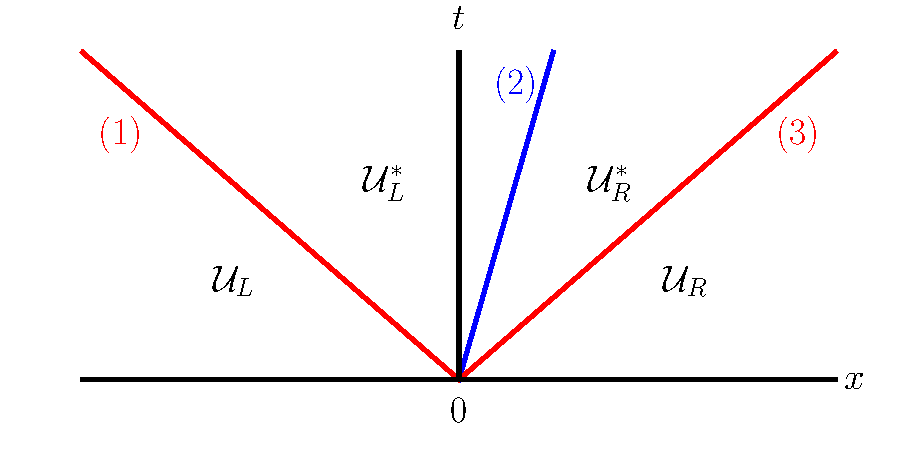
\includegraphics[width=.8\linewidth]{./figures/FV/riemann_solution.pdf}%
    \caption[Structure of the solution to the Riemann problem for Euler equations]{
The structure of the solution to the Riemann problem for Euler equations:
Three waves, (1), (2), and (3), arise from the origin as time evolves.
(2) is always a contact wave, (1) and (3) can be either rarefaction or shock waves in each
case, depending on the initial conditions.\\
The initial states $\U_L$ and $\U_R$ are separated through the waves (1) and (3) from the
two new arising ``star states'' $\U_L^*$ and $\U_R^*$, which themselves are separated by the contact
wave (2).
    }
    \label{fig:riemann-solution}
\end{figure}


It now remains to determine which type of wave those 3 emanating waves are. In order to do so, we
need to look at the eigenvalues $\lambda_i$  and the corresponding eigenvectors
$\mathbf{K}^{(i)}$ of the Jacobian matrix  $\frac{\del \F}{\del \U}$. They are given by

\begin{align}
    &\lambda_1 = v - c_s, &&
    \lambda_2 = v,  &&
    \lambda_3 = v + c_s && \\
    &\mathbf{K}^{(1)} = \begin{pmatrix}
                         1 \\ v - c_s \\ \frac{E + p}{\rho} - v c_s
                        \end{pmatrix} &&
    \mathbf{K}^{(2)} = \begin{pmatrix}
                         1 \\ v \\ \frac{1}{2} v^2
                        \end{pmatrix} &&
    \mathbf{K}^{(3)} = \begin{pmatrix}
                         1 \\ v - c_s \\ \frac{E + p}{\rho} - v c_s
                        \end{pmatrix} &&
\end{align}

We can now see that the $\lambda_2$ characteristic field is always linearly degenerate, i.e.
satisfy eq.~\ref{eq:linear-degenerate-field}:
\begin{align}
  \lambda_2 &= v = \frac{\uc_2}{\uc_1} \\
  \nabla \lambda_2 &= \begin{pmatrix}
                       \frac{\del \lambda_2}{\del \uc_1} \\
                       \frac{\del \lambda_2}{\del \uc_2} \\
                       \frac{\del \lambda_2}{\del \uc_3}
                      \end{pmatrix}
                   =  \begin{pmatrix}
                        -\frac{\uc_2}{\uc_1^2} \\
                        \frac{1}{\uc_1} \\
                        0
                      \end{pmatrix}
                   =  \begin{pmatrix}
                        -\frac{v}{\rho} \\
                        \frac{1}{\rho} \\
                        0
                      \end{pmatrix}
                      \\
 \nabla \lambda_2 \cdot \mathbf{K}^{(2)} &= -\frac{v}{\rho} + \frac{v}{\rho} + 0 = 0
\end{align}

while the other two, $\lambda_1$ and $\lambda_3$, are genuinely non-linear:
\begin{align}
  \lambda_{1,3} &= v \pm c_s = \frac{\uc_2}{\uc_1} \pm c_s \\
  \nabla \lambda_{1,3} &= \begin{pmatrix}
                       \frac{\del \lambda_{1,3}}{\del \uc_1} \\
                       \frac{\del \lambda_{1,3}}{\del \uc_2} \\
                       \frac{\del \lambda_{1,3}}{\del \uc_3}
                      \end{pmatrix}
                   =  \begin{pmatrix}
                        -\frac{\uc_2}{\uc_1^2} \\
                        \frac{1}{\uc_1} \\
                        0
                      \end{pmatrix}
                   =  \begin{pmatrix}
                        -\frac{v}{\rho} \\
                        \frac{1}{\rho} \\
                        0
                      \end{pmatrix}
                      \\
 \nabla \lambda_{1,3} \cdot \mathbf{K}^{(1,3)} &= -\frac{v}{\rho} + \frac{v \pm c_s}{\rho} + 0 \neq
0
\end{align}

They are genuinely non-linear for all energies $E$ and fluid velocities $v$. The vacuum case
$\rho = 0$ will require some special treatment though, which will be discussed later in
Section~\ref{chap:vacuum}.


These considerations tell us the following: The middle wave, associated with $\lambda_2$, will
always be a contact wave, while the other two will either be shocks or rarefactions. Whether the
outer waves are shocks or rarefactions is determined by the new star states $\U_L^*$ and $\U_R^*$.
A model problem containing all three waves is shown in figure \ref{fig:riemann-solved}.
Unfortunately, in order to find the resulting star states $\U_L^*$ and $\U_R^*$ we need to know
which wave type separates them from the outer states $\U_L$ and $\U_R$, respectively, so relations
across the waves, such as the Rankine-Hugeniot relations
\footnote{There are also other very helpful relations, like the Generalized Riemann Invariants,
which have been omitted from this introduction for brevity. In a nutshell, they establish how some
derived quantities change between adjacent states separated by a wave. Under some specific
circumstances, the Generalized Riemann Invariants are constants, and allow us to find relations
between the states.}
(eq.~\ref{eq:rankine-hugeniot}) can be applied correctly. This leaves us with a circular relation:
The specific wave type determines the star states, while the star states determine the wave type.
For this reason, an exact closed form solution for the Euler equations is not available. It is
however possible to make use of an iterative scheme to compute the exact solution numerically,
which is what is at the core of the exact Riemann solver.



\begin{figure}
\centering
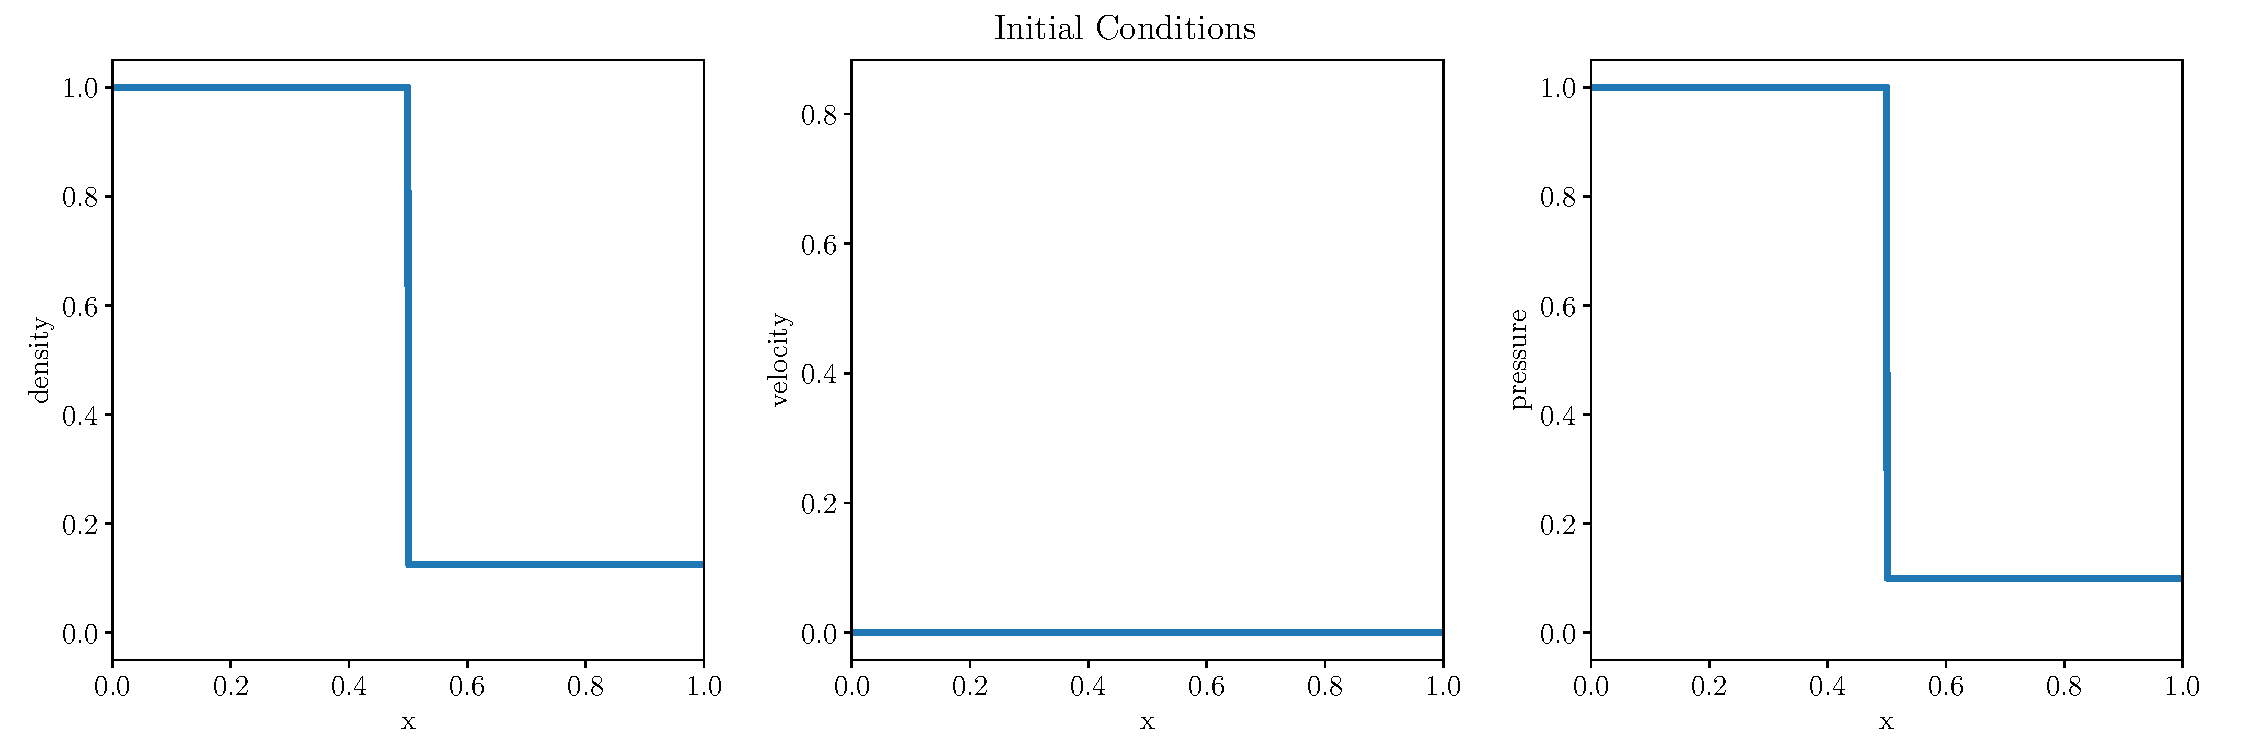
\includegraphics[width=\textwidth]{./figures/FV/riemann_IC.pdf}%
\\
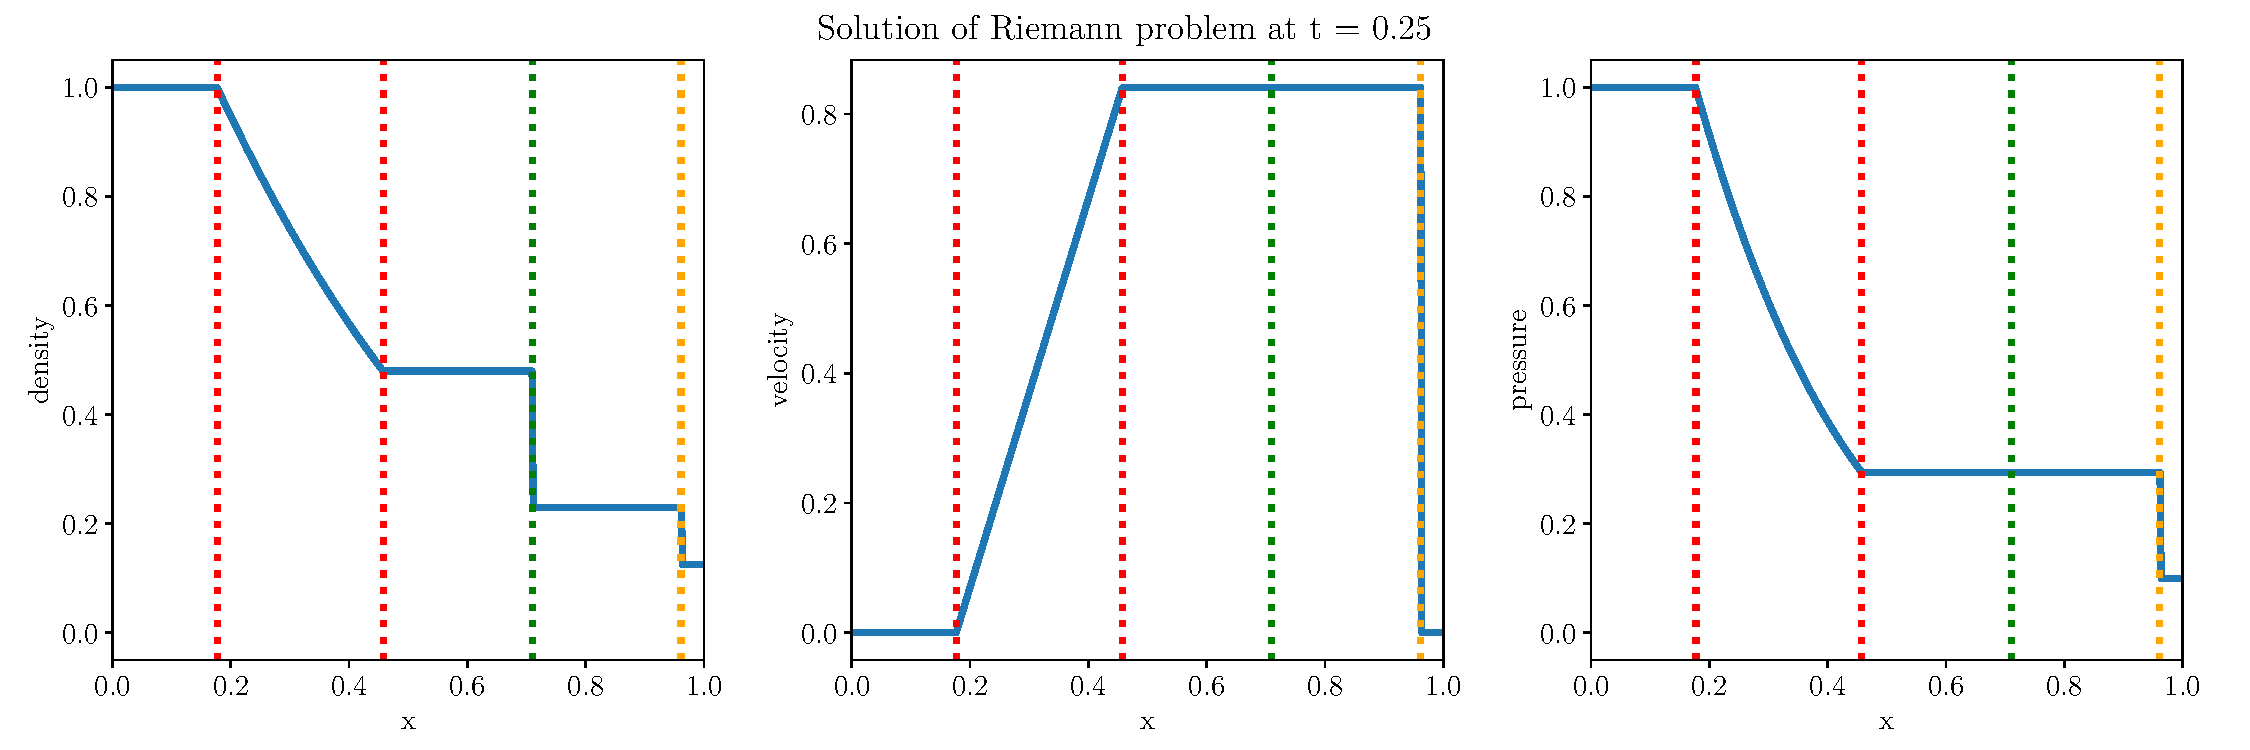
\includegraphics[width=\textwidth]{./figures/FV/riemann_exact_solution.pdf}%
\caption[Sod shock initial conditions and solution]{
    Top row: The initial conditions to a classical Riemann problem, called the Sod shock, in
    arbitrary units.
    Bottom row: The exact solution of the problem at $t = 0.25$. The solution consists of a left
    facing rarefaction wave (between the two red dotted lines), easily recognizable due to being a
    smooth transition, not a jump discontinuity.
    To the right (orange dotted line) is a shock wave, across which all three
    primitive quantities (density, pressure, velocity) change as a jump discontinuity.
    The two waves enclose the third middle wave (green dotted line), which is a contact wave.
    The contact wave is a jump discontinuity just like a shock wave, but only the density changes;
    Velocity and pressure remain constant.
    }%
    \label{fig:riemann-solved}
\end{figure}



A full derivation of the exact Riemann solver is way out of scope for this introduction into the
topic. I refer an interested reader to the works of \citet{toroRiemannSolversNumerical2009}
and \citet{levequeFiniteVolumeMethods2002} for more details. Instead, only an outline of the
derivation and the final result will be discussed.

The outline is as follows: We first establish relations between the four different states $\U_L$,
$\U_L^*$, $\U_R^*$, and $\U_R$ for each permissible wave type between them, which is a contact wave
between $\U_L^*$ and $\U_R^*$, and both shocks and rarefactions between $\U_L$ and $\U_L^*$, and
$\U_R$ and $\U_R^*$, respectively. Experience\footnote{It turns out that using the primitive variables, in particular the pressure $p$ and velocity $v$, is very practical because these two quantities are constant across the middle wave.} shows that a more concise solution can be written in terms of ``primitive variables'' density $\rho$, velocity $v$, and pressure $p$ instead of the
conserved variables density $\rho$, momentum $\rho v$, and energy $E$. Using $\W$ to denote the
state vector of primitive variables, the change of variables is straightforward:

% \begin{align}
% 	&(\rho) = (\rho) &&
% 	(\rho) = (\rho) &&
% 	\\
% 	&(\rho \V) = (\rho) \cdot (\V) &&
% 	(\V) = \frac{(\rho \V )}{(\rho)} &&
% 	\\
% 	&(E) = \frac{1}{2} (\rho) (\V)^2 + \frac{(p)}{\gamma - 1} &&
% 	(p) = (\gamma - 1)  \left((E) - \frac{1}{2} \frac{(\rho \V)^2}{(\rho)} \right) &&
% \end{align}


\begin{align}
    \U &=
        \begin{pmatrix}
        (\rho) \\
        (\rho \V) \\
        (E)
        \end{pmatrix} =
        \begin{pmatrix}
        (\rho) \\
        (\rho) \cdot (\V) \\
        \frac{1}{2} (\rho) (\V)^2 + \frac{(p)}{\gamma - 1}
        \end{pmatrix}
    \\
    \W &=
        \begin{pmatrix}
        (\rho) \\
        (\V) \\
        (p)
        \end{pmatrix} =
        \begin{pmatrix}
        (\rho) \\
        \frac{(\rho \V )}{(\rho)} \\
        (\gamma - 1)  \left((E) - \frac{1}{2} \frac{(\rho \V)^2}{(\rho)} \right)
        \end{pmatrix}
\end{align}


Now let's look at the relations between the states across waves:






%===========================================
\subsubsection{Contact Wave}
%===========================================

It can be shown\footnote{It can be shown using the aforementioned Generalized Riemann Invariants,
which have been omitted for brevity.} that across a contact wave, the pressure and fluid velocity
are constant, i.e.

\begin{align}
	p^*_L &= p^*_R = p^*\\
	v^*_L &= v^*_R = v^*
\end{align}


This means that for the Euler equations, the contact wave is a jump discontinuity in the density
$\rho$ only. For this reason, the star state pressure and velocity will have no index indicating
whether they are the left or right star state, and will be referred to as $p^*$ and $v^*$,
respectively. The contact wave also propagates with velocity $\lambda_2(\U_L^*) = \lambda_2(\U_R^*)
= v^*$.









%===========================================
\subsubsection{Shock Wave}
%===========================================

A shock wave is, just like the contact wave, a jump discontinuity. In contrast to a contact wave
however, all three primitive variables $\rho$, $p$, and $u$ change across a shock wave. The
relations between two states separated by a shock wave can be found using the Rankine-Hugeniot
relations (eq. \ref{eq:rankine-hugeniot}).
Explicitly, if the \emph{leftmost} wave (wave (1) in Fig.~\ref{fig:riemann-solution}) is a shock
wave, for a given star state pressure $p^*$ we have:

\begin{align}
	\rho^*_L &=
		\frac{\frac{p^*}{p_L} + \frac{\gamma - 1}{\gamma+1}}{\frac{\gamma - 1}{\gamma+1}
\frac{p^*}{p_L} + 1} \rho_L \label{eq:rho-shock-first}\\
	v^* &=
		v_L - \frac{p^* - p_L}{\sqrt{\frac{p^* + B_L}{A_L}}}
		= v_L - f_L(p^*) \label{eq:velocity-shock-left} \\
    f_L(p^*) &=
        \frac{p^* - p_L}{\sqrt{\frac{p^* + B_L}{A_L}}} \\
	A_L &=
		\frac{2}{(\gamma + 1) \rho_L}\\
	B_L &=
		\frac{\gamma - 1}{\gamma + 1} p_L
\end{align}

The shock speed is
\begin{align}
	S_L = u_L - c_{s,L} \left[\frac{\gamma + 1}{2 \gamma} \frac{p^*}{p_L} + \frac{\gamma -
1}{2\gamma} \right]^{\half} \label{eq:shock-left-speed}
\end{align}

where $c_{s,L}$ is the sound speed in the left state $U_L$.



For a \emph{right shock wave}, i.e. when wave (3) is a shock wave, for a given star state
pressure $p^*$ we have the relations

\begin{align}
	\rho^*_R &=
		\frac{\frac{p^*}{p_R} + \frac{\gamma - 1}{\gamma+1}}{\frac{\gamma - 1}{\gamma+1}
\frac{p^*}{p_R} + 1} \rho_R \\
	v^* &=
		v_R + \frac{p^* - p_R}{\sqrt{\frac{p^* + B_R}{A_R}}}
		= v_R + f_R(p^*) \label{eq:velocity-shock-right} \\
    f_R(p^*) &=
        \frac{p^* - p_R}{\sqrt{\frac{p^* + B_R}{A_R}}} \\
	A_R &=
		\frac{2}{(\gamma + 1) \rho_R}\\
	B_R &=
		\frac{\gamma - 1}{\gamma + 1} p_R
\end{align}

and the shock speed is
\begin{align}
	S_R = v_R + c_{s,R} \left[\frac{\gamma + 1}{2 \gamma} \frac{p^*}{p_R} + \frac{\gamma -
1}{2\gamma} \right]^{\half} \label{eq:shock-right-speed}
\end{align}

where $c_{s,R}$ is the sound speed in the right state $U_R$.








%===========================================
\subsubsection{Rarefaction Wave}
%===========================================

Rarefaction waves are smooth transitions, not infinitesimally thin jump discontinuities.
This makes them really easy to spot in the solutions of Riemann problems (compare with Fig.~
\ref{fig:riemann-solved}).
% Across rarefactions, entropy is conserved.

The rarefaction waves are enclosed by the head and the tail of the wave, between which we have a
smooth transition which is called the ``fan''.
The head is the ``front'' of the wave, i.e. the part of the wave that gets furthest away from the
origin as time progresses.
The tail is the ``back'' of the wave, i.e. the part of the wave that stays closest to the origin as
time progresses.

If we have a \emph{left-facing} rarefaction, i.e. if wave (1) is a rarefaction wave,
the wave speeds of the head, $S_{HL}$, and the tail, $S_{TL}$, are given by

\begin{align}
	S_{HL} &= u_L - c_{s,L}\\
	S_{TL} &= u^* - c_{s,L}^*\\
	c_{s,L}^*  &= c_{s,L} \left( \frac{p^*}{p_L} \right) ^ \frac{\gamma - 1}{2 \gamma}
\end{align}

The star state $\W_L^*$ for a given pressure $p^*$ is determined by

\begin{align}
	\rho^*_L &=
		\rho_L \left( \frac{p^*}{p_L} \right) ^ \frac{1}{\gamma}\\
	v^* &=
		v_L - \frac{2 c_{s,L}}{\gamma - 1} \left[ \left( \frac{p^*}{p_L} \right) ^ \frac{\gamma -
1}{2 \gamma} -1  \right]
		= v_L - f_L(p^*) \label{eq:velocity-rarefaction-left} \\
    f_L(p^*) &=
        \frac{2 c_{s,L}}{\gamma - 1} \left[ \left( \frac{p^*}{p_L} \right) ^ \frac{\gamma - 1}{2
\gamma} -1  \right]\\
\end{align}


where and $c_{s,L}$ is the sound speed in the left state $U_L$.



The solution \emph{inside} the rarefaction fan, i.e. in regions where $S_{HL} \leq \frac{x}{t}
\leq S_{TL}$, is

\begin{align}
	\rho_{\text{fan}, L} &=
		\rho_L \left[ \frac{2}{\gamma + 1} + \frac{\gamma - 1}{\gamma + 1} \frac{1}{c_{s,L}}
\left(v_L - \frac{x}{t}\right) \right] ^ \frac{2}{\gamma -1 } \label{eq:rho-rarefaction-fan-left}\\
	v_{\text{fan}, L} &=
		\frac{2}{\gamma + 1} \left[ \frac{\gamma - 1}{2} v_L + c_{s,L} + \frac{x}{t}  \right] \\
	p_{\text{fan}, L} &=
		p_L \left[ \frac{2}{\gamma + 1} + \frac{\gamma - 1}{\gamma + 1} \frac{1}{c_{s,L}} \left(v_L
- \frac{x}{t}\right) \right] ^ \frac{2 \gamma}{\gamma -1} \label{eq:pressure-rarefaction-fan-left}
\end{align}









If we have a \emph{right-facing rarefaction}, i.e. if wave (3) is a rarefaction wave, we have

\begin{align}
	\rho^*_R &=
		\rho_R \left( \frac{p^*}{p_R} \right) ^ \frac{1}{\gamma}\\
	v^* &=
		v_R - \frac{2 c_{s,R}}{\gamma - 1} \left[ 1 - \left( \frac{p^*}{p_R} \right) ^ \frac{\gamma
- 1}{2 \gamma}  \right]
		= v_R + f_R(p^*)
    \label{eq:velocity-rarefaction-right}
\\
    f_R(p^*) &= \frac{2 c_{s,R}}{\gamma - 1} \left[ 1 - \left( \frac{p^*}{p_R} \right) ^
\frac{\gamma -
1}{2 \gamma}  \right]
\end{align}

where $c_{s,R}$ is the sound speed in the left state $U_R$.


The wave speeds of the head, $S_H$, and the tail, $S_T$, for the left facing wave are
\begin{align}
	S_{HR} &= v_R + c_{s,R}\\
	S_{TR} &= v^* + c^*_{s,R}\\
	c^*_{s,R}  &= c_{s,R} \left( \frac{p^*}{p_R} \right) ^ \frac{\gamma - 1}{2 \gamma}
\end{align}




Finally, the solution inside the rarefaction fan, i.e. in regions where $S_{HL} \leq \frac{x}{t}
\leq S_{TL}$, is

\begin{align}
	\rho_{\text{fan}, R} &=
		\rho_R \left[ \frac{2}{\gamma + 1} - \frac{\gamma - 1}{\gamma + 1} \frac{1}{c_{s,R}}
\left(v_R - \frac{x}{t}\right) \right] ^ \frac{2}{\gamma -1 } \label{eq:rho-rarefaction-fan-right}
\\
	v_{\text{fan}, R} &=
		\frac{2}{\gamma + 1} \left[ \frac{\gamma - 1}{2} v_R - c_{s,R} + \frac{x}{t}  \right]
    \label{eq:velocity-rarefaction-fan-right}
\\
	p_{\text{fan}, R} &=
		p_R \left[ \frac{2}{\gamma + 1} - \frac{\gamma - 1}{\gamma + 1} \frac{1}{c_{s,R}} \left(v_R
- \frac{x}{t}\right) \right] ^ \frac{2 \gamma}{\gamma -1} \label{eq:pressure-rarefaction-fan-right}
\end{align}











%===========================================
\subsubsection{Which wave type do we have?}
%===========================================


As noted before, the middle wave (wave (2) in Fig.~\ref{fig:riemann-solution}) is always a
contact wave, while the other two waves are any combination of rarefaction and/or shock wave.
It turns out that the condition for a rarefaction or shock wave is remarkably simple:

For the left wave (wave (1)):

\begin{align}
	p^* > p_L: && &\quad \text{ (1) is a shock wave}\\
	p^* \leq p_L: && &\quad \text{ (1) is a rarefaction wave}
\end{align}

and for the right wave (wave (3)):

\begin{align}
	p^* > p_R: && & \quad \text{ (3) is a shock wave} \\
	p^* \leq p_R: && & \quad \text{ (3) is a rarefaction wave}
\end{align}

A way of understanding these conditions is to again consider the behavior of the characteristics,
and to take into account that the pressure of an fluid has no preferential direction. So if the
pressure in the star region is greater than the pressure across an outer wave, it'll ``push'' the
fluid from the star region stronger than in the outer regions. Interpreting this ``push'' as the
behavior of the characteristics of the fluid, the characteristics of the star regions will have a
steeper slope, and eventually cross with the characteristics from the outer regions on the $x-t$
plane. This is precisely the condition of converging characteristics required for shock waves in a
compressive region.








%===========================================
\subsubsection{Solution for $p^*$}
%===========================================

The final missing element to have a complete exact solution to the Riemann problem for the Euler
equations is an expression how to obtain $p^*$, the pressure in the star region, depending on the
initial conditions $\W_L$ and $\W_R$. We make use of the fact that $p^*$ and $v^*$ are constant
across the star region states $\W_L^*$ and $\W_R^*$. For both shock and rarefaction waves on either
side, we have equations for $v^*$ depending on the outer states  $\W_L$ and $\W_R$ and $p^*$ (eqns.
\ref{eq:velocity-shock-left}, \ref{eq:velocity-shock-right}, \ref{eq:velocity-rarefaction-left},
and \ref{eq:velocity-rarefaction-right}). By setting $v^*_L - v^*_R = 0$, which must hold across
the contact wave, we obtain the equation

\begin{align}
	f(p^*, \W_L, \W_R) \equiv f_L(p^*, \W_L) + f_R(p^*, \W_R) + (v_R - v_L) = 0
\label{eq:riemann-pressure-equation}
\end{align}

with

\begin{align}
	f_{L,R} &=
		\begin{cases}
			(p^* - p_{L,R}) \left[ \frac{A_{L,R}}{p^* + B_{L,R}} \right]^{\frac{1}{2}}
				& ~\text{ if } ~ p^* > p_{L,R} ~ \quad \text{(shock)} \\
			\frac{2 c_{s,L,R}}{\gamma - 1} \left[ \left( \frac{p^*}{p_{L,R}} \right)^ \frac{\gamma
-1}{2 \gamma} - 1 \right]
				& ~\text{ if } ~ p^* \leq p^*_{L,R} ~ \quad \text{(rarefaction)}
\label{eq:riemann-pstar}\\
		\end{cases} \\
	A_{L,R} &=
		\frac{2}{(\gamma + 1) \rho_{L,R}}\\
	B_{L,R} &=
		\frac{\gamma - 1}{\gamma + 1} p_{L,R}
\end{align}


Since the expressions for $f_{L,R}$ are analytical, we can also compute their derivatives w.r.t.
$p^*$:

\begin{align}
	\frac{\del f_{L,R}}{\del p^*} &=
		\begin{cases}
			\left[
                \frac{A_{L,R}}{p^* + B_{L,R}}
            \right]^{\frac{1}{2}} \left( 1 - \frac{1}{2}
            \frac{p^* - p_{L,R}}{p + B_{L,R}} \right)
				& ~\text{ if } ~ p^* > p_{L,R} ~ \quad \text{(shock)} \\
			\frac{a_{L,R}}{\gamma p_{L,R}}
			\left( \frac{p^*}{p_{L,R}} \right)^ \frac{-(\gamma+1)}{2 \gamma}
				& ~\text{ if } ~ p^* \leq p_{L,R} ~ \quad \text{(rarefaction)}
\label{eq:riemann-pstar-dp}\\
		\end{cases}
\end{align}

giving the complete derivative of eq.~\ref{eq:riemann-pstar}:

\begin{align}
  \frac{\del}{\del p^*} f(p^*, \W_L, \W_R)= \frac{\del f_L(p^*, \W_L)}{\del p^*} + \frac{\del
f_{R}(p^*, \W_R)}{\del p^*} \ ,
\end{align}


and make use of it to find the $p^*$ that solves eq.~\ref{eq:riemann-pstar} using the iterative
Newton-Raphson method. The method prescribes that the $n + 1$-th iteration is determined by

\begin{align}
	p^*_{n+1} = p^*_n - \frac{f(p^*_n, \W_L, \W_R)}{\frac{\del}{\del p^*}f(p*_n, \W_L, \W_R)}
\end{align}


and is re-iterated until it converges, i.e. when the relative pressure change

\begin{align}
	\frac{|p_k - p_{k+1}|}{\frac{1}{2} | p_k + p_{k+1} | } < \epsilon
\end{align}

where $\epsilon$ is some tolerance, e.g. $10^{-6}$. To begin the iteration, a first guess $p_0^*$
is necessary. Taking the average pressure:

\begin{align}
	p_0^* = \frac{1}{2} (p_L + p_R)
\end{align}

gives acceptable results. A better first guess, i.e. a guess that typically leads to fewer required
iteration steps for the method to converge, is by taking the solution for the star state pressure
of the linearized primitive variable Riemann solver (see
Appendix~\ref{app:riemann-primitive-variables}):

\begin{align}
	p_{PV} &=
        \frac{1}{2} (p_L + p_R) - \frac{1}{8} (v_R - v_L)(\rho_L + \rho_R)(c_{s,L} + c_{s,R})\\
	p_0^* &= \max(\epsilon, p_{PV})
\end{align}


With this, the exact Riemann solver is complete. A method to obtain the star state pressure $p^*$
is given, and with the pressure known, the outer wave types are determined. The exact star states,
$\W_L^*$ and $\W_R^*$ can then be determined by using the appropriate relations for the
corresponding wave type, which are given by
eqns.~\ref{eq:rho-shock-first}~-~\ref{eq:pressure-rarefaction-fan-right}.












%====================================================================
\subsubsection{Sampling the Solution}
%====================================================================


With the exact solver readily available, the final task is to find the solution at some desired
point $(x, t)$. This can be achieved by sampling the solution. Assuming all the star region state
variables are computed, then all four states $\U_L$, $\U_L^*$, $\U_R^*$, and $\U_R$ are known. What
is left to do is to determine in which region the point $(x, t)$ is located. This is done by
comparing $x/t$ with the wave velocities: If $x / t < v^*$, then the point $(x, t)$ must be located
in the left region, i.e. in either $\U_L$ or $\U_L^*$. Further comparison of $x / t$ with the wave
speed of the left wave, which is either a shock or a rarefaction, determines whether $(x, t)$ is in
$\U_L$ or $\U_L^*$. If the left wave is a rarefaction, then another possible solution is for $(x,t)$
to be located inside the rarefaction fan instead. The analogous distinction process is performed if
$(x, t)$ is located in the right region. A full flow chart of decision making and finally which
relations to use is shown in figure \ref{fig:sampling-solution}.


\begin{sidewaysfigure}
	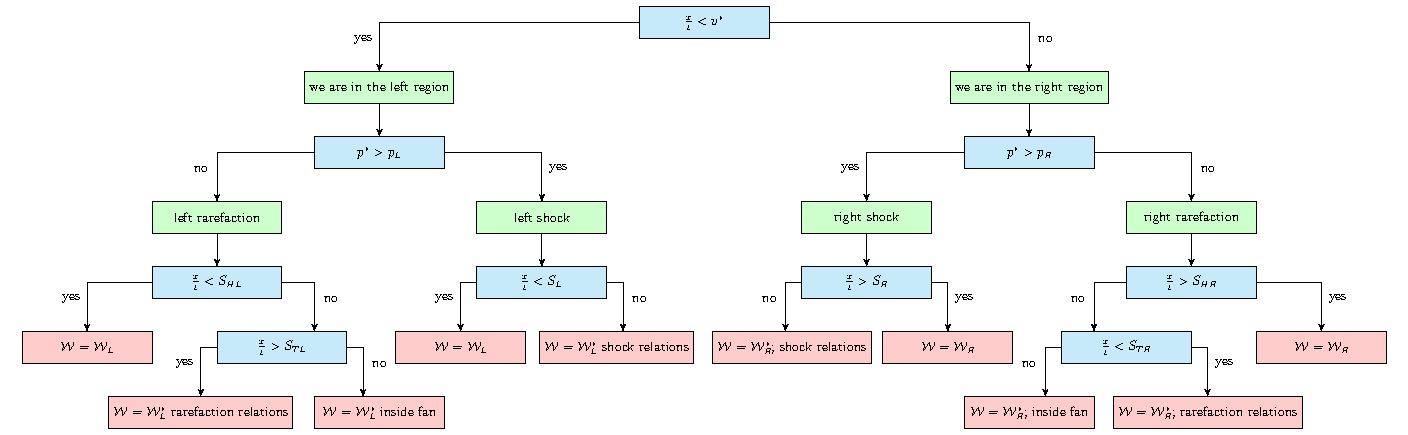
\includegraphics[width=\textheight]{./figures/FV/tikz/sampling_the_solution.pdf}%
	\caption[Flowchart on sampling the solution]{Flow chart to sample the solution of the Riemann
problem for the Euler equations at a given point $(x, t)$.
		\label{fig:sampling-solution}
	}
\end{sidewaysfigure}










%====================================================================
\subsection{Approximate Solvers}\label{chap:riemann-approximate}
%====================================================================


As mentioned before, the solution of the Riemann problem is at the heart of finite volume fluid
dynamics methods. It needs to be solved over and over again at every time step and between every
pair of interacting cells. For example, if a three dimensional simulation volume is divided up in
only 128 cells of equal size in each dimension, it would require $6.29 \times 10^6$ Riemann
problems to be solved \emph{each time step}, assuming that each interacting pair of cells requires
the solution of only one Riemann problem.\footnote{Some methods, like the MUSCL-Hancock scheme,
require more than one Riemann problem to be solved per interaction per cell in order to increase
the accuracy of the numerical method. More details are given in Section \ref{chap:MUSCL-Hancock}}



Given that the exact solver requires iterations in order to find the pressure of the star states
$p^*$, it can become a considerable computational expense. In order to cut some costs, approximate
non-iterative Riemann solvers have been developed. While they only provide approximate solutions,
tests show that they are indeed sufficiently accurate to be made use of in actual simulations. How
exactly the Riemann solvers are used in finite volume methods to solve the Euler equations will be
the topic of Chapters~\ref{chap:godunov}~and~\ref{chap:higher-order-schemes}, while the influence
of approximate Riemann solvers on simulations will be discussed in
Section~\ref{chap:godunov-application}. In what follows, some popular approximate Riemann solvers
are introduced.







%=================================================================================
\subsubsection{Two-Rarefaction Riemann Solver (TRRS)}\label{chap:riemann-trrs}
%=================================================================================

The Two-Rarefaction Riemann Solver (TRRS) is a modification of the exact Riemann solver. The
approach used to skip over the iteration for the star state pressure $p^*$ is to assume that both
outer waves are rarefaction waves, and to use that assumption to get an expression for $p^*$ and
$v^*$, the pressure and velocity in the star region, respectively. The expressions are given by:

\begin{align}
	\beta &\equiv
		\frac{\gamma - 1}{2 \gamma} \\
	v^* &=
		\frac{
			\frac{2}{\gamma - 1} \left[\left(\frac{p_L}{p_R} \right) ^ \beta - 1\right]+
\frac{v_L}{c_{s,L}} \left(\frac{p_L}{p_R} \right) ^ \beta  + \frac{v_R}{c_{s,R}}
		}{
			\frac{1}{c_{s,R}} + \frac{1}{c_{s,L}}\left(\frac{p_L}{p_R} \right) ^ \beta
		} \\
	p^* &=
		\frac{1}{2} \left[
			p_R \left[ \frac{\gamma - 1}{2 c_{s,R}} (v^* - v_R) + 1 \right] ^ \frac{1}{\beta} +
			p_L \left[ \frac{\gamma - 1}{2 c_{s,L}} (v_L - v^*) + 1 \right] ^ \frac{1}{\beta}
		\right] \label{eq:pstar-trrs} \\
		&=
		\left[
			\frac{ c_{s,L} + c_{s,R} - \frac{\gamma - 1}{2} (v_R - v_L)}{\frac{c_{s,L}}{p_L^\beta}
+         \frac{c_{s,R}}{p_R^\beta}}
		\right] ^ \frac{1}{\beta}
\end{align}


To remain consistent with the two-rarefaction assumption, the star state densities can be obtained
using
\begin{align}
    \rho^*_{L,R} = \rho_{L,R} \left(\frac{p^*}{p_{L,R}} \right)^{\frac{1}{\gamma}}
\end{align}

However, an improved solution can be obtained by using the approximation only to estimate the star
state pressure, $p^*$, and then proceeding in the same manner as the exact solver does: By
determining what type of waves the two outer waves are based on $p^*$, and using the appropriate
relations for the wave types to determine the other star state variables and wave velocities.














%=============================================================================
\subsubsection{Two-Shock Riemann Solver (TSRS)}\label{chap:riemann-tsrs}
%=============================================================================


Similar to the TRRS solver, the Two-Shock Riemann Solver (TSRS) is also a modification of the exact
Riemann solver. As the name suggests, in order to determine the star region pressure $p^*$, it is
assumed a priori that both the left and right waves are going to be shock waves.


The equation for the pressure in the star region (eq. \ref{eq:riemann-pressure-equation}) then is given by

\begin{align}
	f(p) &= (p - p_L) g_L(p) + (p - p_R) g_R(p) + v_R - v_L = 0 \label{eq:riemann-pressure-tsrs} \\
	g_{L,R}(p) &= \left[ \frac{A_{L,R}}{p + B_{L,R}} \right] ^{\half} \\
	A_{L,R} &=
		\frac{2}{(\gamma + 1) \rho_{L,R}}\\
	B_{L,R} &=
		\frac{\gamma - 1}{\gamma + 1} p_{L,R}
\end{align}

Unfortunately, this approximation does not lead to a closed form solution, and a further
approximation is needed. A first estimate for the pressure, $p_0$, is used as the argument for
$g_{L,R}(p)$ in eq.~\ref{eq:riemann-pressure-tsrs} to get a better approximation for $p^*$:

\begin{align}
	p^* = \frac{g_L(p_0) p_L + g_R(p_0)p_R - (v_R - v_L)}{g_L(p_0) + g_R(p_0)} \label{eq:pstar-tsrs}
\end{align}

The star region velocity which is consistent with the two-shock assumption is given by

\begin{align}
	v^*  = \frac{1}{2} (v_L + v_R) + \frac{1}{2} \left[ (p^* - p_R) g_R(p_0) - (p^* - p_L) g_L(p_0)
\right]
\end{align}


A good choice for $p_0$ is coming from the solution for the star state pressure of the linearized
primitive variable Riemann solver (Appendix~\ref{app:riemann-primitive-variables}):

\begin{align}
	p_{PV} &= \frac{1}{2} (p_L + p_R) - \frac{1}{8} (v_R - v_L)(\rho_L + \rho_R)(c_{s,L} +
c_{s,R})\\
	p_0 &= \max(0, p_{PV})
\end{align}

Just as was the case for the TRRS solver, an improved solution can be found by only using the TSRS
approximation to estimate $p^*$ and determining the other star region quantities using the
relations of the exact Riemann solver.







%====================================================================
\subsubsection{HLLC Solver}\label{chap:riemann-hllc}
%====================================================================

The HLLC (Harten, Lax, van Leer, contact) Riemann solver is derived by assuming that the solution
consists of three waves that are jump discontinuities. The three waves are traveling with speeds
denoted by $S_L$, $S^*$, and $S_R$, respectively. In the context of the Euler equations, it is an
improved version of the HLL (Harten, Lax, van Leer) solver, which doesn't take into account a middle
contact wave. While the missing contact wave of the HLL approach is sub-optimal for the Euler
equations, it can be a good approximation for other systems of hyperbolic conservation laws that
only consist of two equations. Indeed, the approximate HLL solver will be used later in the context
of the moments of the equation of radiative transfer in Section~\ref{chap:riemann-rt}.

% Alternative: \ref{chap:transport-step}

To find relations across the three contact discontinuities which the HLLC approach assumes, the
Rankine-Hugeniot relations (eq.~\ref{eq:rankine-hugeniot}) can be applied. Further relations can be
found by integrating the conservation law equations over both a space and time interval, and using
that integral to obtain the integrated average value in the star region. The solution takes the form

\begin{align}
	\U(x, t) = \begin{cases}
		\U_L ~~~~ &\text{ if }		~~	\frac{x}{t} \leq S_L \\
		\U^*_L ~~~~ &\text{ if }	~~  S_L \leq \frac{x}{t} \leq S^* \\
		\U^*_R ~~~~ &\text{ if }	~~	S^* \leq \frac{x}{t} \leq S_R \\
		\U_R ~~~~ &\text{ if }		~~	S_R \leq \frac{x}{t} \\
	\end{cases}
\end{align}

By additionally using properties of the contact wave from the exact solver, i.e. the fact that $p^*
= p^*_L = p^*_R$ and $v^* = v^*_L = v^*_R = S^*$, an expression for $S^*$ can be found that only
depends on the initial left and right states:

\begin{align}
	S^* &=
		\frac{p_R - p_L  + \rho_L v_L (S_L - v_L) - \rho_R v_R (S_R - v_R)}
			{\rho_L (S_L - v_L) - \rho_R (S_R - v_R) } \label{eq:hllc-sstar}
\end{align}

and ultimately

\begin{align}
	\U^*_{L,R} &=
		\rho_{L,R} \frac{ S_{L,R} - v_{L,R}}{S_{L,R} - S^*}
		\begin{pmatrix}
			1\\
			S^*\\
			\frac{E_{L,R}}{\rho_{L,R}} + (S^* - v_{L,R}) \left( S^* +
\frac{p_{L,R}}{\rho_{L,R}(S_{L,R} - v_{L,R})} \right)
		\end{pmatrix} \\
	\F^*_{L,R} &=
		\F_{L, R} + S_{L,R} ( \U^*_{L,R} - \U_{L,R} )
\end{align}

It remains to find estimates for the left and right wave speeds, $S_L$ and $S_R$.
There are multiple ways to get good and robust estimates. A very simple one is:

\begin{align}
	S_L  &= v_L - c_{s,L} q_L \\
	S_R  &= v_R + c_{s,R} q_R \\
	q_{L,R} &=
		\begin{cases}
			1	~~~~ & \text{ if } p^* \leq p_{L,R} ~~~~ \text{(rarefaction)}\\
			\sqrt{1 + \frac{\gamma + 1}{2 \gamma} \left(\frac{p^*}{p_{L,R}} - 1 \right)}
			~~~~ & \text{ if } p^* > p_{L,R} ~~~~ \text{(shock)}\\
		\end{cases} \\
	p^* &= \max(0, p_{PV})\\
	p_{PV} &= \frac{1}{2} (p_L + p_R) - \frac{1}{8} (v_R - v_L)(\rho_L + \rho_R)(c_{s,L} + c_{s,R})
\label{eq:pstar-pv}.
\end{align}


A better estimate using an adaptive wave speed estimate method can be obtained.
In order to do so, first  the primitive variable solution for the star state pressure $p^*$
following eq. \ref{eq:pstar-pv} is computed (see Appendix~\ref{app:riemann-primitive-variables}).
That first guess is kept as long as the ratio $\frac{p_{max}}{p_{min}}$ is small enough (typically
$\sim 2$), where $p_{max} = \max \{ p_L, p_R \}$ and $p_{min} = \min \{ p_L, p_R \}$. Furthermore,
we also demand that $p_{min} \leq p_{PV} \leq p_{max}$. Should one of these two conditions not be
satisfied, then we switch to the star state solutions of other approximate Riemann solvers: If
$p_{PV} \leq p_{min}$, then it's reasonable to expect two rarefactions to form, and applying the
star state estimates of the Two Rarefaction Riemann Solver (TRRS, eq. \ref{eq:pstar-trrs}) is a good
choice. Otherwise, we expect at least one shock should be present, so the star state estimates of
the Two Shock Riemann Solver (TSRS, eq. \ref{eq:pstar-tsrs}) will likely provide a better estimate.





%====================================================================
\subsubsection{On the Accuracy of Approximate Riemann Solvers}
%====================================================================

To conclude the chapter on approximate Riemann solvers, let's have a look at how accurate the
solutions of the approximate solvers are. In what follows, Riemann problems are solved using the
exact solver as well as the approximate TRRS, TSRS, and HLLC solvers. All quantities are in
arbitrary units, and the tests are performed in one dimension using the \meshhydro code's option
to run it as a standalone Riemann solver. For each test, an initial left and right state are
specified, which are separated at the position $x = 0.5$. The solution is obtained using the various
Riemann solvers, and then sampled over the region $x \in [0, 1]$ over $10^3$ equally spaced points.
It is important to note that the solution the Riemann solvers provide for the star
region states do not evolve over time. The only thing that changes over time is the front of the
waves, but the states remain the same for all $t > 0$. This can be seen well in
Figure~\ref{fig:approximate-riemann-left-blast-wave}, where the solution at two different times is
shown. Hence it makes little sense to compare how well the approximate solvers perform as time
evolves, and the results for each test are shown for only a single time.


Figure~\ref{fig:approximate-riemann-sod-test} shows the results of the so-called ``Sod test''
Riemann problem with initial conditions

\begin{align}
    \rho_L = 1 && v_L = 0 && p_L = 1 \label{eq:sod-test-ICs} \\
    \rho_R = 0.125 && v_R = 0 && p_R = 0.1      \nonumber
\end{align}

The exact solution consists of a left-facing rarefaction and a right facing shock. The TRRS
solver gives a result which is nearly identical to the exact solution, which makes sense given the
prominent rarefaction wave in the solution. All solvers except the HLLC find approximately the
same pressure in the star region, which indicates that all of them will ``identify'' the correct
wave type when sampling the solution.
Both the HLLC and the TSRS solver find nearly identical velocities in the star region compared to
each other, but offset compared to the exact solution, which is due to the similarity they share in
how the star region velocity (and pressure) is initially estimated.
The HLLC solver, which by construction can't handle the
smooth transition of the rarefaction since it assumes waves are only jump discontinuities, has some
trouble getting the correct solution on the left side of the problem, and the errors propagate
throughout the star region. A further noticeable feature of the HLLC solver is that it's the only
one that has a pressure change over the star region, i.e. across the contact wave. This is not in
agreement with what the properties of the contact wave dictate, and is a consequence of the way the
outer wave speeds $S_L$ and $S_R$ are estimated. To avoid an iterative scheme (which is the
entire point of approximate solvers), either the identical pressure over the star region can be
enforced, or the correct relations across the waves with velocities $S_L$ and $S_R$ can be
enforced. But to have both the pressure and the relations across the wave be consistent can't be
done without an iterative scheme.



\begin{figure}
\centering
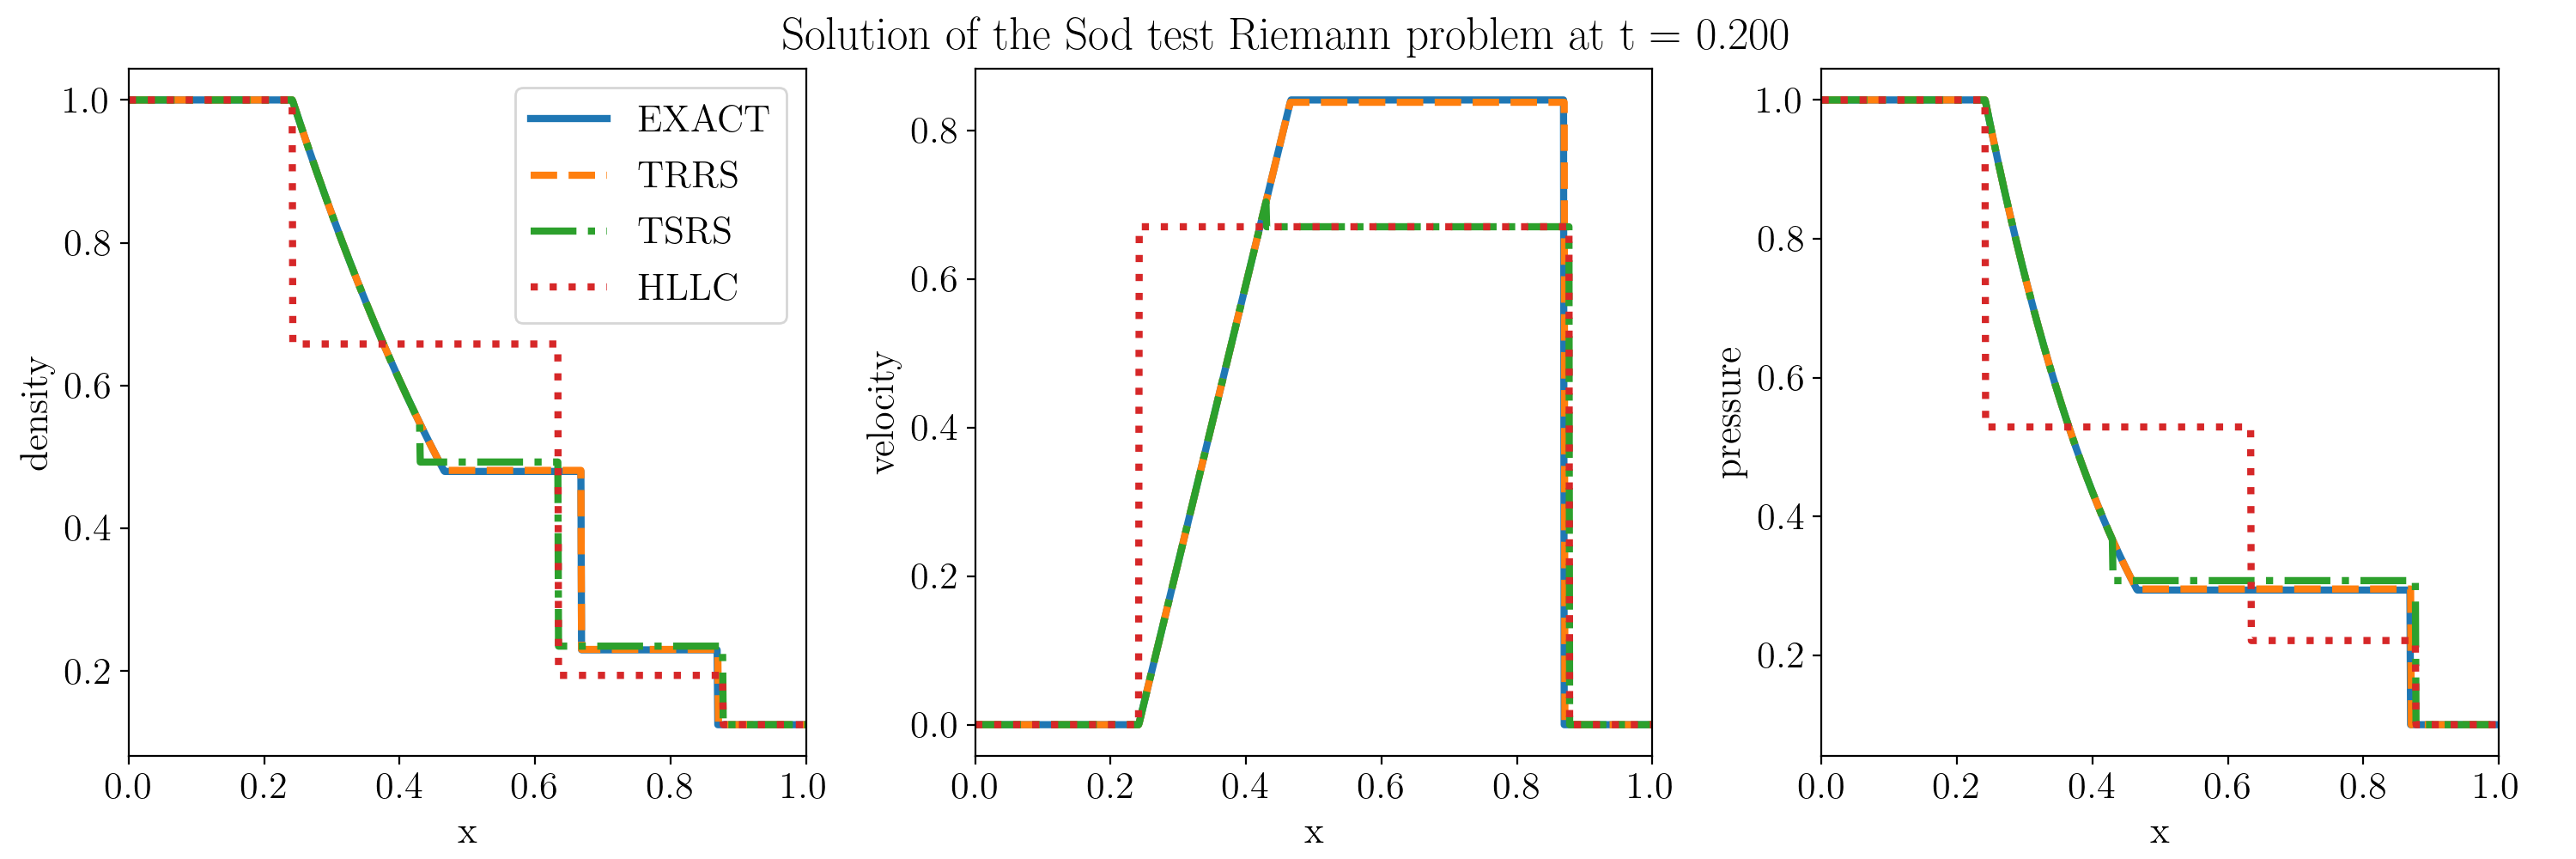
\includegraphics[width=\textwidth]{
./figures/FV/approximate_riemann_solvers/riemann-approximate-sod_test-0.200.png} %
\caption[Sod test solution with approximate Riemann solvers]{
    The solution to the Sod test (eq. \ref{eq:sod-test-ICs}) using different approximate and the
    exact Riemann solver. The exact solution consists of a left-facing rarefaction and a right
    facing shock.
    }%
\label{fig:approximate-riemann-sod-test}
\end{figure}




Figure~\ref{fig:approximate-riemann-left-blast-wave} shows the results of the so-called ``Left
blast wave'' Riemann problem with initial conditions

\begin{align}
    \rho_L = 1 && v_L = 0 && p_L = 1000 \label{eq:left-blast-wave-ICs} \\
    \rho_R = 1 && v_R = 0 && p_R = 0.01      \nonumber
\end{align}

Similarly to the Sod test, the solution consists of a left-facing rarefaction and a right facing
shock. However in this test the shock is much stronger and much more prominent. The compression
wave travels from the left to the right. Figure~\ref{fig:approximate-riemann-left-blast-wave}
depicts the solution at two times to showcase this behavior.

In this test, the TSRS solver gives a result very close to the exact solution. The HLLC solver
handles the jump discontinuities on the right hand side of the solution quite well, but struggles
again with the rarefaction on the left. The TRRS solver struggles this time around to get close to
the exact solution, which makes sense due to the prominent shock present, which is contrary to its
underlying two-rarefaction assumption.

\begin{figure}
\centering
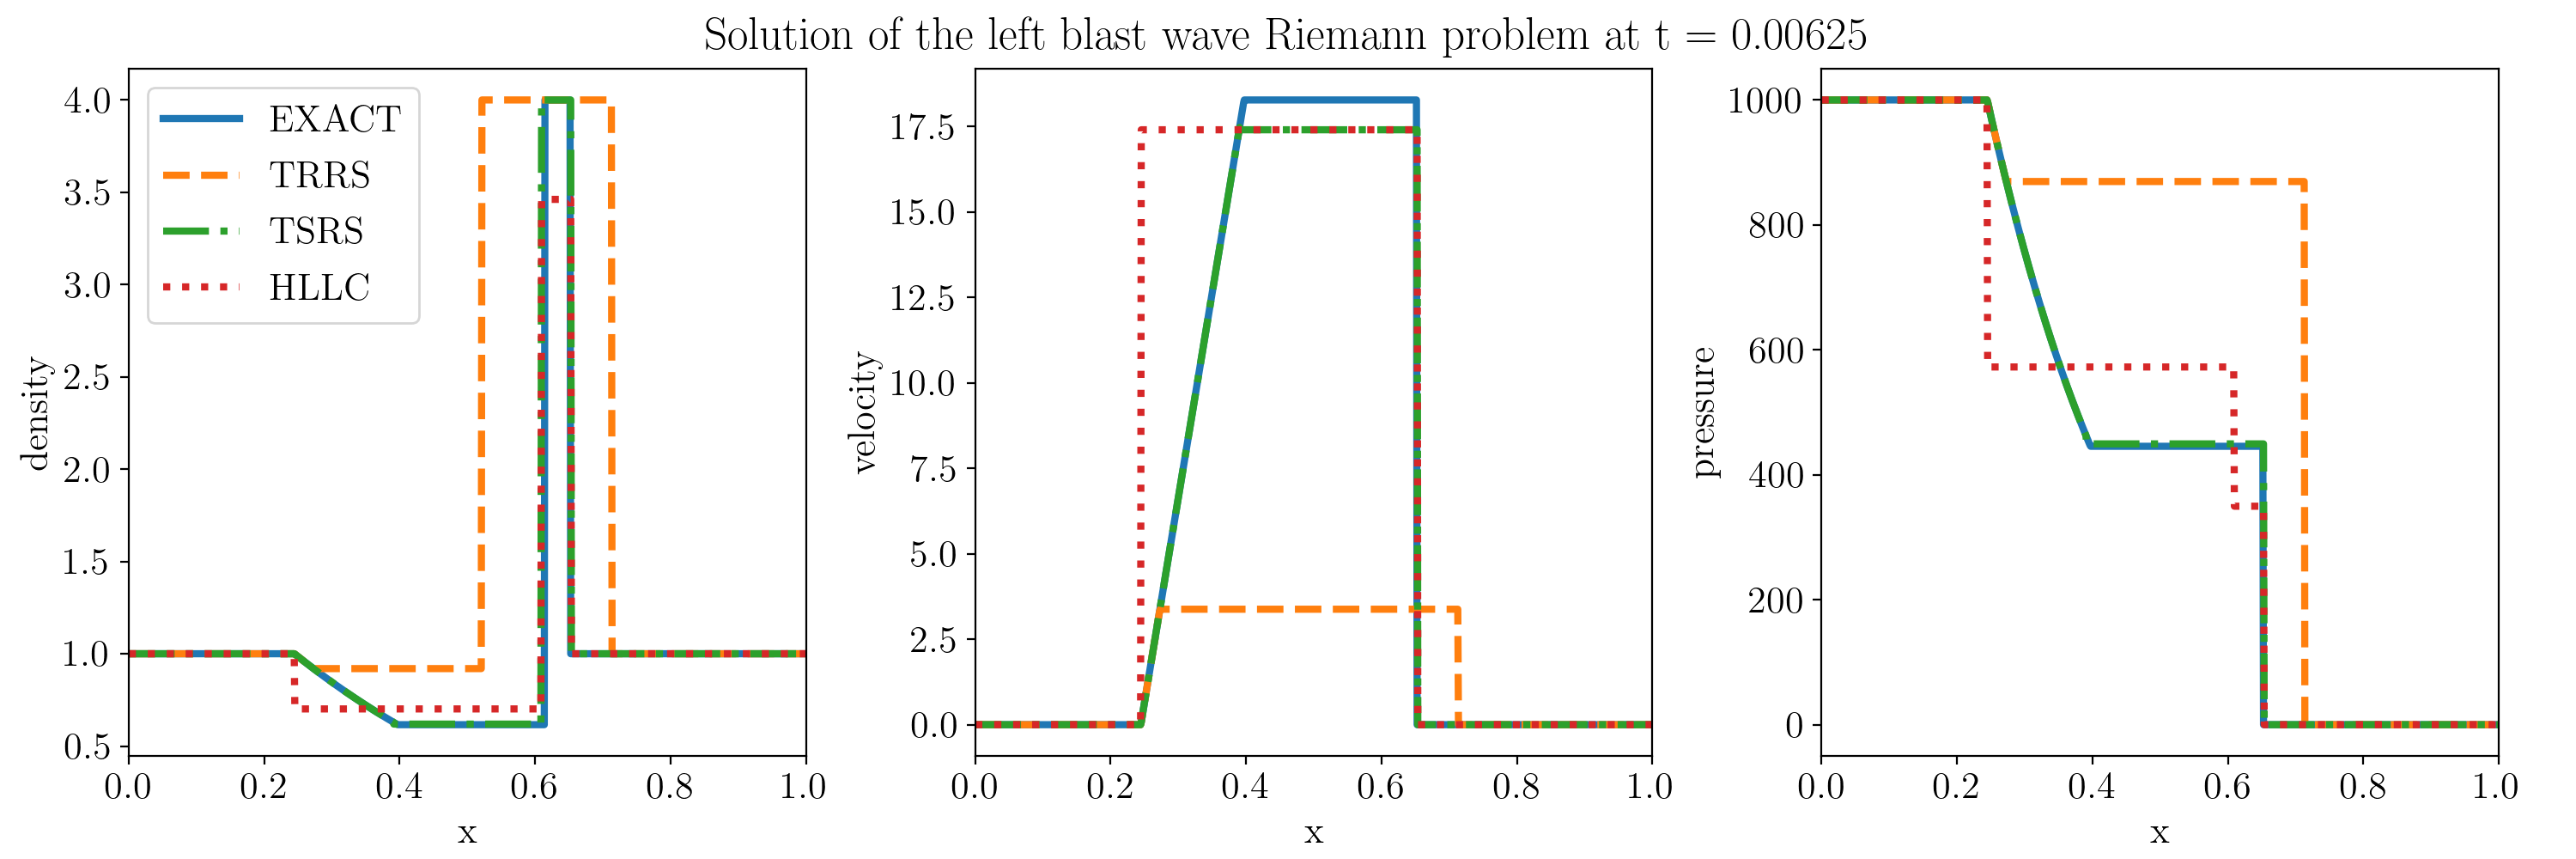
\includegraphics[width=\textwidth]{
./figures/FV/approximate_riemann_solvers/riemann-approximate-left_blast_wave-0.006.png} %
\\
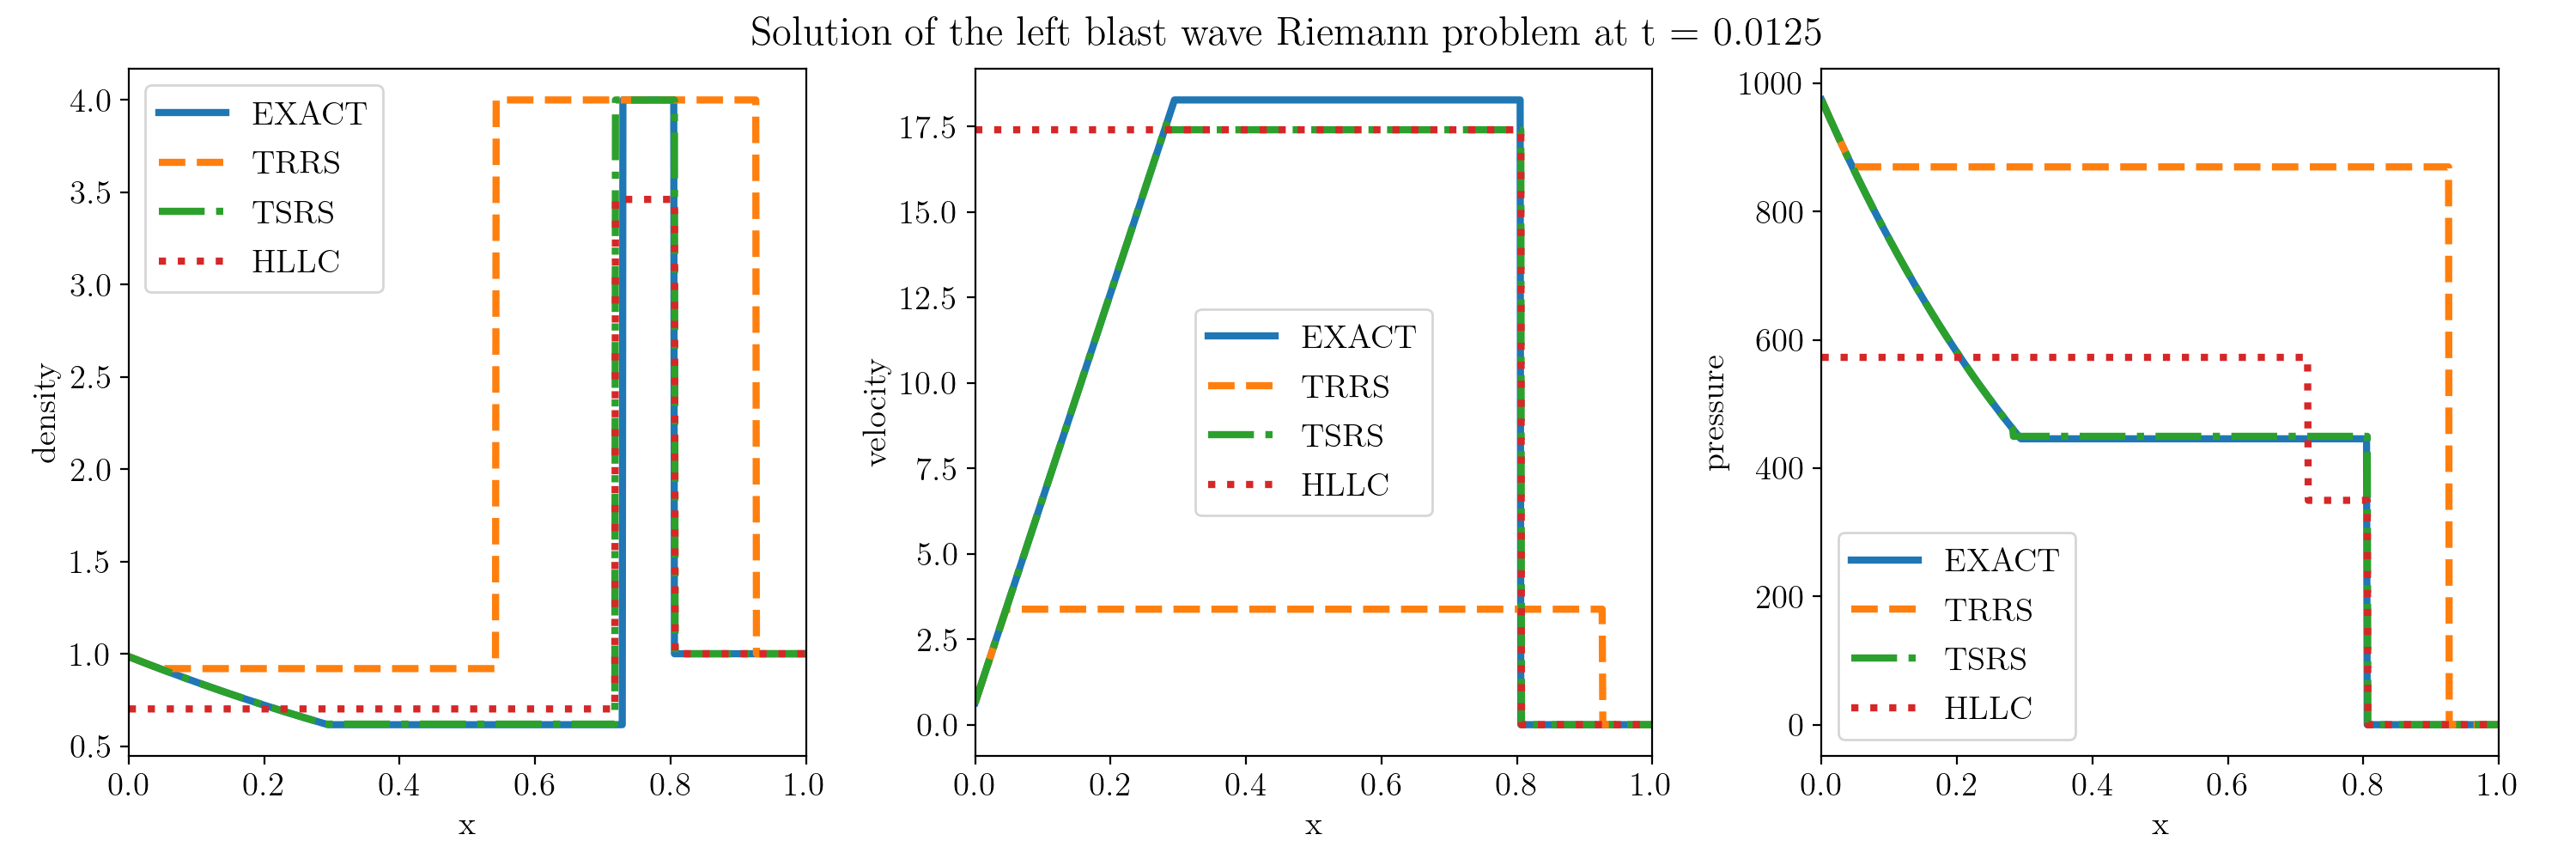
\includegraphics[width=\textwidth]{
./figures/FV/approximate_riemann_solvers/riemann-approximate-left_blast_wave-0.013.png} %
\caption[Left blast wave solution with approximate Riemann solvers]{
    The solution to the left blast wave test (eq. \ref{eq:left-blast-wave-ICs}) using different
    approximate and the exact Riemann solver. The exact solution consists of a left-facing
    rarefaction and a right facing shock. To showcase the wave originating on the left side of the
    interface (located at $x=0.5$) and traveling to the right, the solution is shown at two
    different times $t = 0.00625$ and $t = 0.0125$.
    }%
    \label{fig:approximate-riemann-left-blast-wave}
\end{figure}


A further test, shown in Figure~\ref{fig:approximate-riemann-two-shocks} where all the approximate
solvers struggle to reproduce the exact solution is the two-shock test, given by the initial
conditions

\begin{align}
    \rho_L = 5.99924 && v_L = 19.5975 && p_L = 460.894 \label{eq:two-shock-ICs} \\
    \rho_R = 5.99242 && v_R = -6.19633 && p_R = 46.095      \nonumber
\end{align}

As the name suggests, the solution consists of two shock waves, one on either side of the central
contact wave. While it can be expected from the TRRS solver to have issues reproducing the exact
result, both the HLLC and the TRRS solvers struggle as well. They fail to obtain a close enough
initial guess for the central region, and the offsets from the exact solution consequently
propagate into the resulting states and wave speeds. A silver lining is that once again all solvers
were at least able to ``identify'' that both outer waves are shock waves.

\begin{figure}
\centering
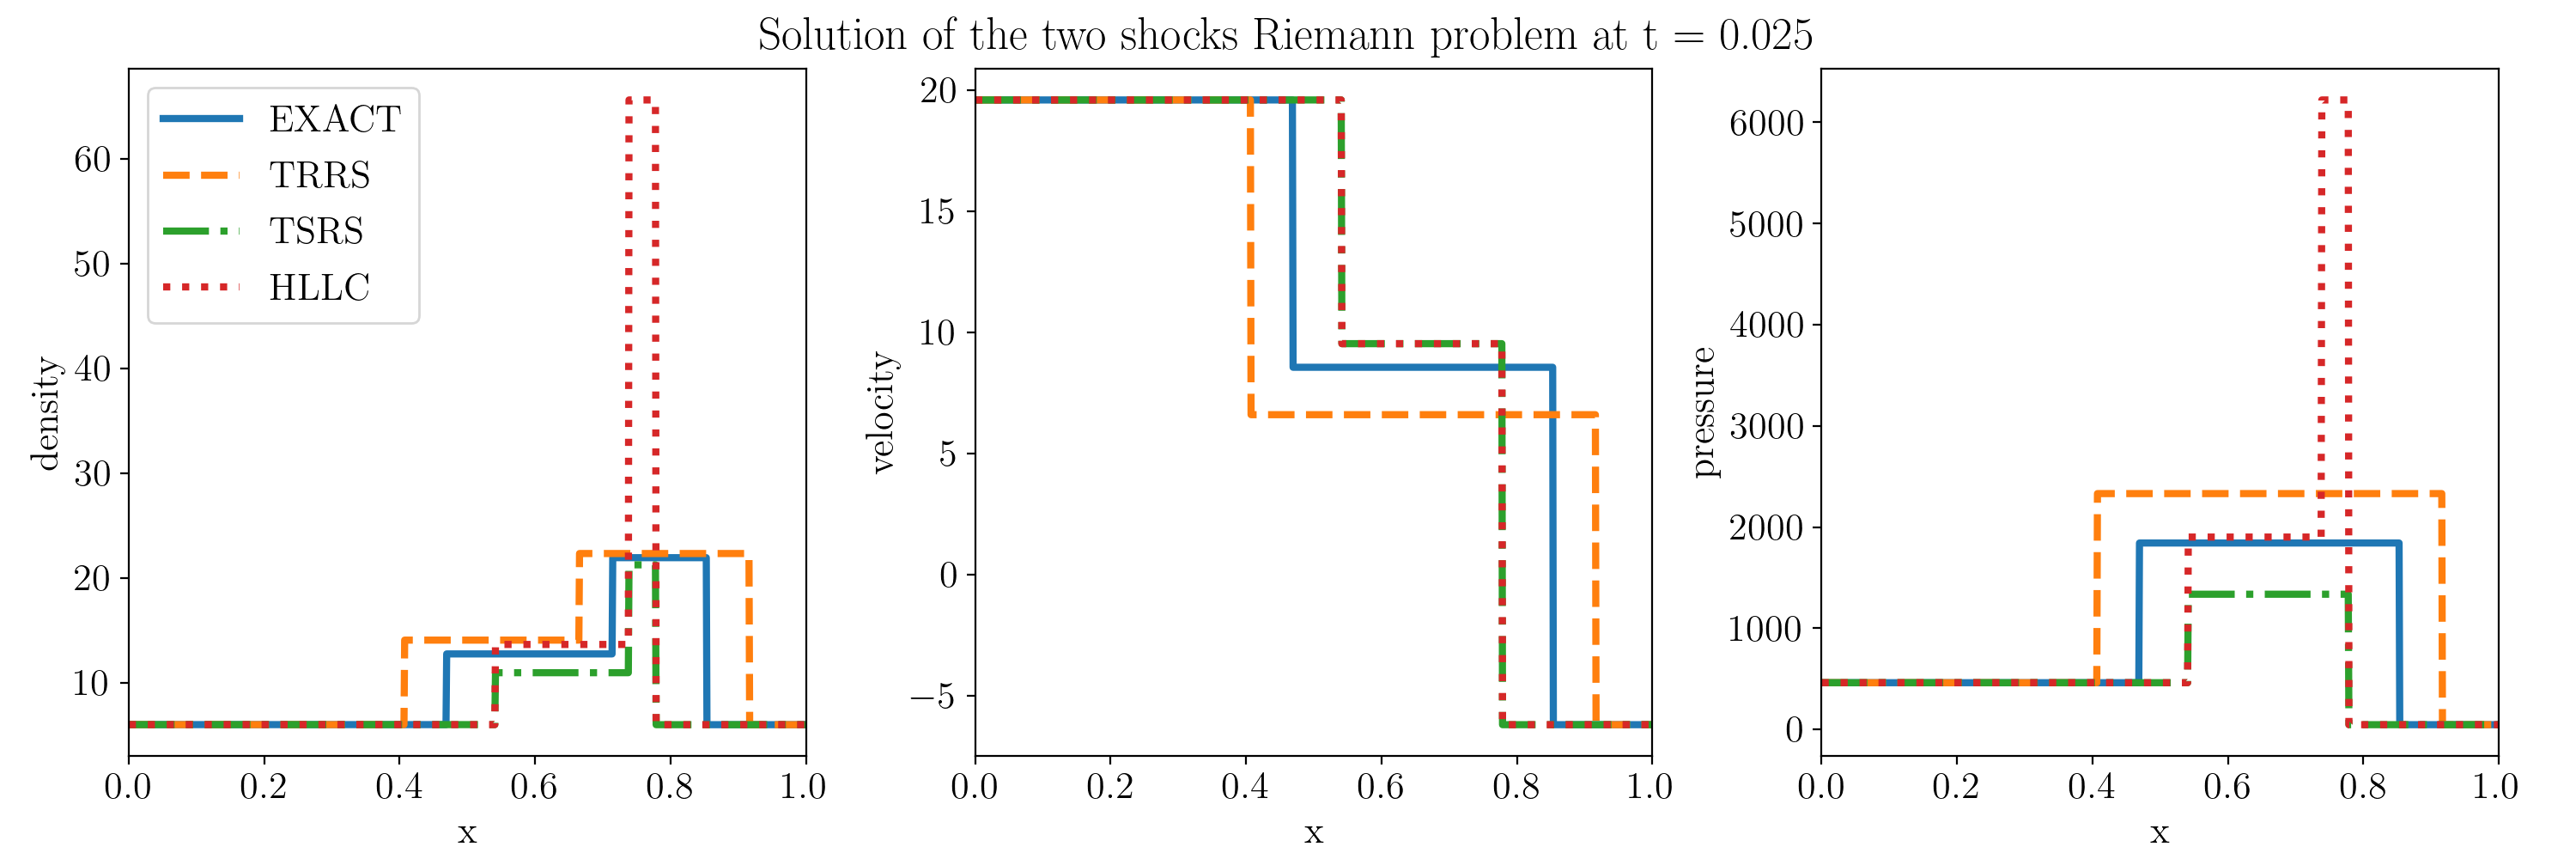
\includegraphics[width=\textwidth]{
./figures/FV/approximate_riemann_solvers/riemann-approximate-two_shocks-0.025.png} %
\caption[Two shocks solution with approximate Riemann solvers]{
    The solution to the two shock test (eq. \ref{eq:left-blast-wave-ICs}) using different
    approximate and the exact Riemann solver. The exact solution consists of a two shocks on either
    side of the contact wave.
    }%
    \label{fig:approximate-riemann-two-shocks}
\end{figure}


The errors of the results that approximate solvers yield may seem troubling at first, but it turns
out that when employed as solvers in simulations, those errors aren't as severe as the results
shown may suggest. Indeed the results aren't off by orders of magnitudes. The most extreme
deviations in these examples are off by a factor of $\sim 2 - 3$. Note however that these are errors
on the solution of the Riemann problems specified by the initial conditions only. In simulations,
the the state of the fluid is evolved over  many small time steps, typically much smaller than the
end times shown in the previous plots. This means that initially large errors can get smoothed out
over subsequent time steps. Additionally, numerical effects like diffusion, and the application of
flux and slope limiters for higher order schemes lead to the errors resulting from approximate
solvers being in many cases negligible. The influence of the approximate Riemann solvers is shown
in e.g. Section~\ref{chap:godunov-application}. Which Riemann solver to choose depends on factors
like what physical case is going to be simulated, as well as specifics of the underlying method.
For example, very smooth flows will likely have little to no shocks, and a TRRS solver could be
beneficial. Conversely, in turbulent flows or in cases where a lot of energy is being injected into
the gas, the TRRS solver can be practical. For a general purpose application, the HLLC solver is
recommended, or even the exact one, if one can afford it.










%====================================================================
\subsection{Dealing with Vacuum}\label{chap:vacuum}
%====================================================================

A final topic that requires some discussion is the special case of vacuum. Vacuum is characterized
by the condition $\rho = 0$. Given the equation of state for ideal gas (eq.
\ref{eq:equation-of-state}), it follows that $E = 0$ as well.
The structure of the solution to the Riemann problem is different when vacuum is present. The
general solution structure of three waves separating four distinct states doesn't hold any longer:
There is no more star region. Instead, a non-vacuum state will be separated from the vacuum state
through a rarefaction fan, which in turn is separated from the vacuum state through a contact wave
which overlaps with the tail of the rarefaction. A shock wave cannot be adjacent to a vacuum state,
which can be shown using the Rankine-Hugeniot relations: Let a left non-vacuum state $\U_L =
(\rho_L, v_L, E_L)^T$ with the corresponding flux $\F_L = (\rho_L v_L, \rho_L v_L^2 + p_L, (E_L +
p_L) v_L)^T$ be adjacent to a vacuum state $\U_0 = (\rho_0, v_0, E_0)^T$ with the corresponding flux
$\F_0 = (\rho_0, \rho v_0^2 + p_0, (E_0 + p_0) v_0)^T$. Assuming the left and the vacuum state are
separated by a jump discontinuity with velocity $S$, then the Rankine-Hugeniot conditions give us

\begin{align}
    \F_L - \F_0 &= S (\U_L - \U_0) \\
    \rho_L v_L - \rho_0 v_0  &= S( \rho_L - \rho_0) \label{eq:vacuum1} \\
    \rho_L v_L^2 + p_L - \rho_0 v_0^2 - p_0  &= S( \rho_L v_L - \rho_0 v_0) \label{eq:vacuum2} \\
    v_L (E_L + p_L) - v_0 (E_0 + p_0) &= S( E_L - E_0) \label{eq:vacuum3}
\end{align}

By assuming $\rho_0 = E_0 = 0$ and that $v_0$ is finite, we obtain


\begin{align}
    \rho_L v_L  &= S \rho_L \label{eq:vacuum4} \\
    \rho_L v_L^2 + p_L - p_0  &= S \rho_L v_L \label{eq:vacuum5} \\
    v_L (E_L + p_L) - v_0 p_0 &= S E_L \label{eq:vacuum6}
\end{align}

These three equations give us the following relations:

\begin{align}
    v_L &= S = v_0 \label{eq:vacuum-v0}\\
    p_L &= p_0 \label{eq:vacuum-p0}
\end{align}

The equal pressures across the wave in eq.~\ref{eq:vacuum-p0} indicate that a shock wave is not a
possible solution, since a shock wave requires unequal pressures between the waves. However,
this solution allows for a contact wave. Eq.~\ref{eq:vacuum-v0} states that the wave will propagate
at the velocity dictated by the non-vacuum state, which physically makes sense if one interprets the
wave as the boundary between the vacuum and the non-vacuum states whose position evolves over time.
Given eq.~\ref{eq:vacuum-p0}, the pressure at the contact wave must be the same as the pressure in
the vacuum state, which is zero. This means that for any left state $\U_L$, the only applicable
solution for $t > 0$ between the left state itself and the contact wave must be a rarefaction fan,
since $p_L \geq p_0$. This leads to the conclusion that the solution structure must be that the
initial left state $\U_L$ is separated from the vacuum state through a rarefaction fan, which ends
with a contact wave overlapping with its tail at the vacuum state.

With the structure of the solution known, the previously found relations can be applied again, and
the solution to the Riemann problem with a left non-vacuum state $\U_L$ and right vacuum state
$\U_0$ is given by

\begin{align}
    S_{vac, L} &= v_L + \frac{2 c_{s,L}}{\gamma - 1} \\
    \U_{L, \text{ with vacuum }}(x,t) &=
        \begin{cases}
            \U_L & \quad \text{ if } \frac{x}{t} \leq v_L - c_{s,L} \\
            \U_{L, \text{inside fan}} & \quad \text{ if } v_L - c_{s,L} < \frac{x}{t} < S_{vac, L}
\\
            \U_{vac} & \quad \text{ if } \frac{x}{t} \geq S_{vac, L}\\
        \end{cases}
\end{align}

The solution $\U_{L, \text{inside fan}}$ inside the rarefaction fan is given by
eqns.~\ref{eq:rho-rarefaction-fan-left}~-~\ref{eq:pressure-rarefaction-fan-left}.
The inverse case, with a right non-vacuum state $\U_R$ and a left vacuum state $\U_{vac}$, the
solution is given by

\begin{align}
    S_{vac, R} &= v_R - \frac{2 c_{s,R}}{\gamma - 1} \\
    \U_{R, \text{ with vacuum }} &=
        \begin{cases}
            \U_{vac} & \quad \text{ if } \frac{x}{t} \leq S_{vac, R}\\
            \U_{R, \text{inside fan}} & \quad \text{ if } S_{vac, R} < \frac{x}{t} < v_R + c_{s,R}\\
            \U_R & \quad \text{ if } \frac{x}{t} \geq v_R + c_{s,R} \\
        \end{cases}
\end{align}

The solution $\U_{R, \text{inside fan}}$ inside the rarefaction fan is given by
eqns.~\ref{eq:rho-rarefaction-fan-right}~-~\ref{eq:pressure-rarefaction-fan-right}.





In certain cases, with both the left and the right state being non-vacuum states, vacuum
can be generated in central regions of the solution. This can occur when the difference between the
left and right fluid velocities have the opposite direction and are too high for the material to
keep up, generating a vacuum between the two initial states as time evolves. The structure of the
solution contains a left-facing wave connected to a central vacuum region over a rarefaction fan,
and a second left-facing rarefaction fan that connects the central vacuum region with the
right-facing wave. This scenario is shown in Figure~\ref{fig:vacuum-generating}.  To find an
explicit solution, we can make use us the fact that
there must be two rarefaction tails, with speeds $S_{vac,L}$ and $S_{vac,R}$, respectively, just
like in the vacuum-adjacent cases before. The only difference is that now there are two of them.
For two rarefactions fans to develop, $S_{vac, L} \leq S_{vac, R}$ must hold, and hence a condition
for a vacuum generating case can be written as

\begin{align}
    \Delta v_{crit} \equiv \frac{2 c_{s,L}}{\gamma - 1 } + \frac{2 c_{s,R}}{\gamma - 1 } \leq v_R -
v_L \label{eq:vacuum-generating-condition}
\end{align}

If a Riemann problem, like in Figure~\ref{fig:vacuum-generating}, satisfies
condition~\ref{eq:vacuum-generating-condition}, then the full solution is given by

\begin{align}
    \U_{\text{vacuum generating}} =
        \begin{cases}
            \U_{L, \text{ with vacuum }} & \quad \text{ if } \frac{x}{t} \leq S_{vac, L}\\
            \U_{vac} & \quad \text{ if } S_{vac, L} < \frac{x}{t} <  S_{vac, R}\\
            \U_{R, \text{ with vacuum }} & \quad \text{ if } \frac{x}{t} \geq S_{vac, R} \\
        \end{cases}
\end{align}






\begin{figure}
\centering
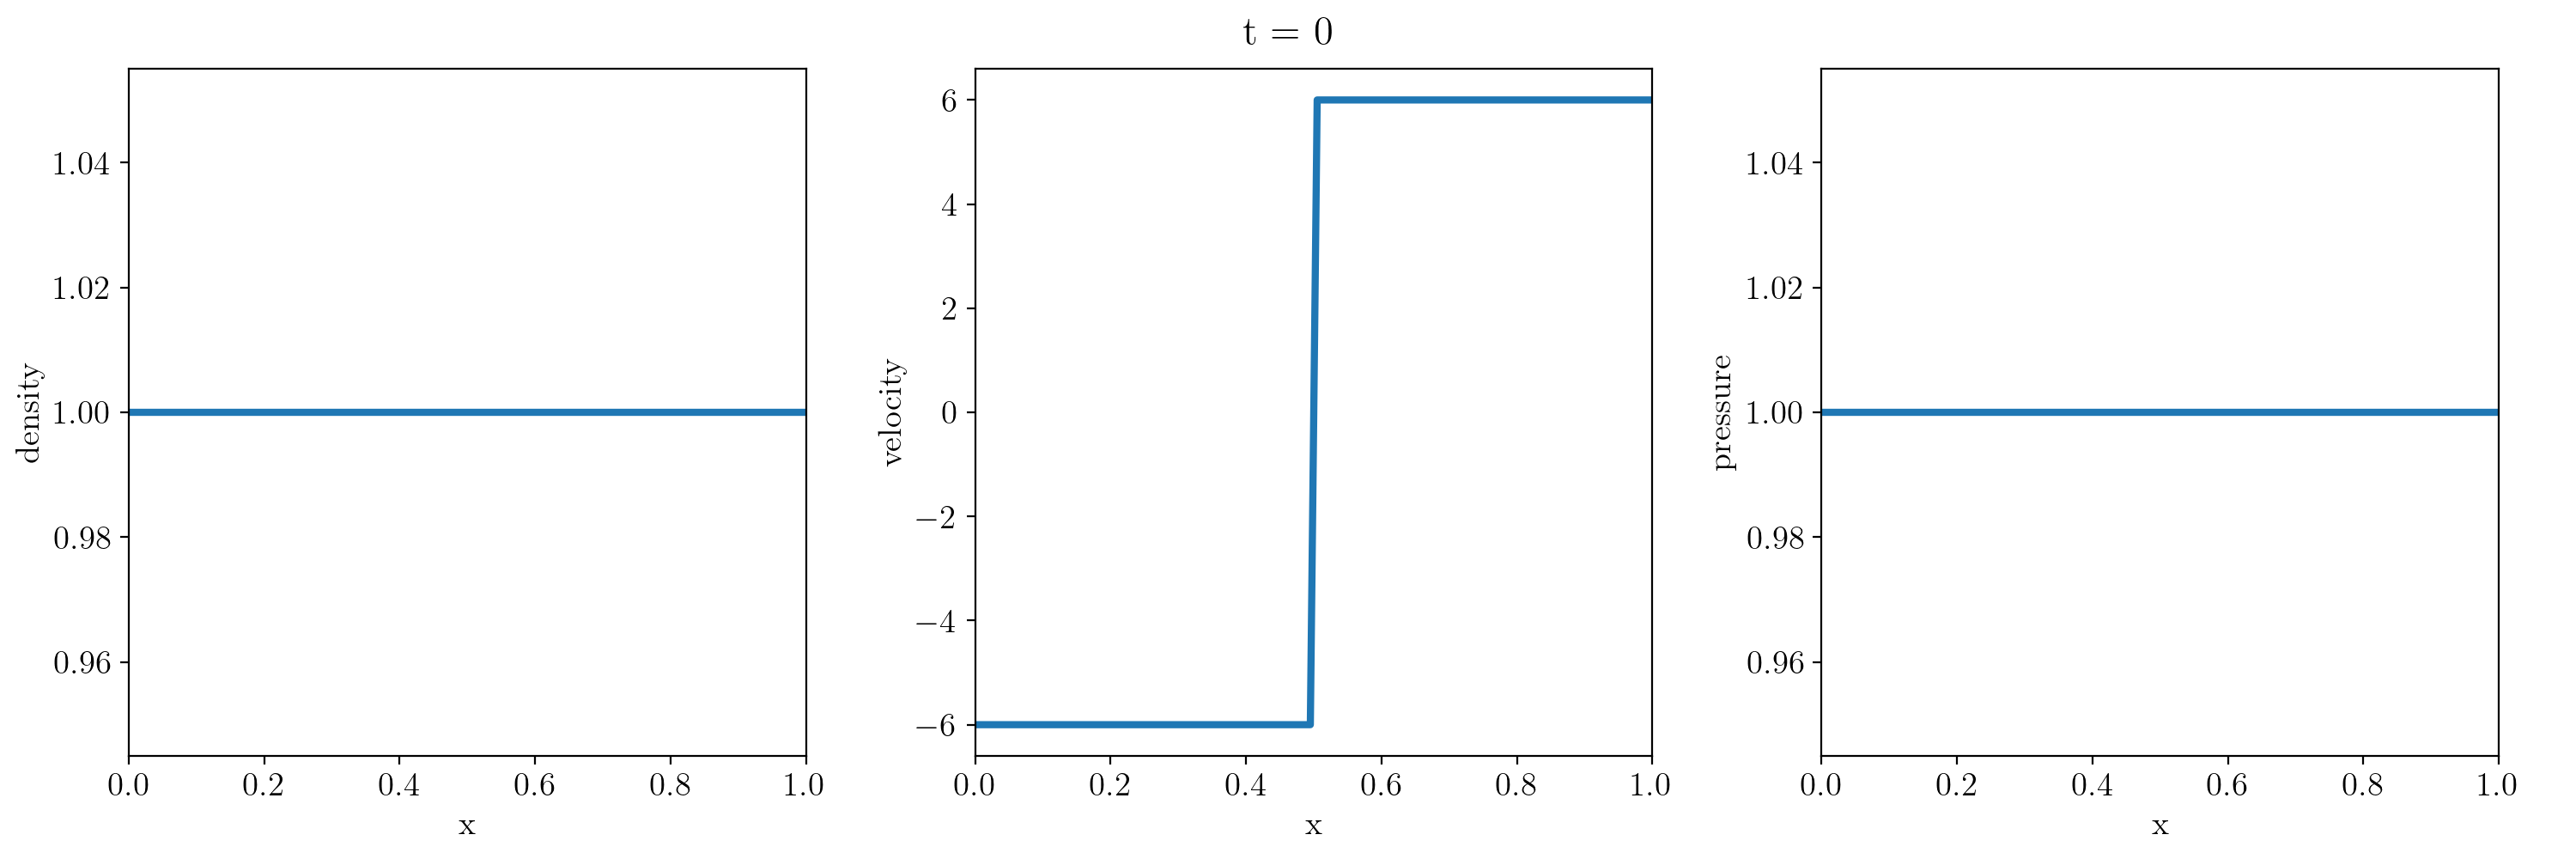
\includegraphics[width=\textwidth]{
./figures/FV/vacuum_generating_ICs/vacuum_generating.png} %
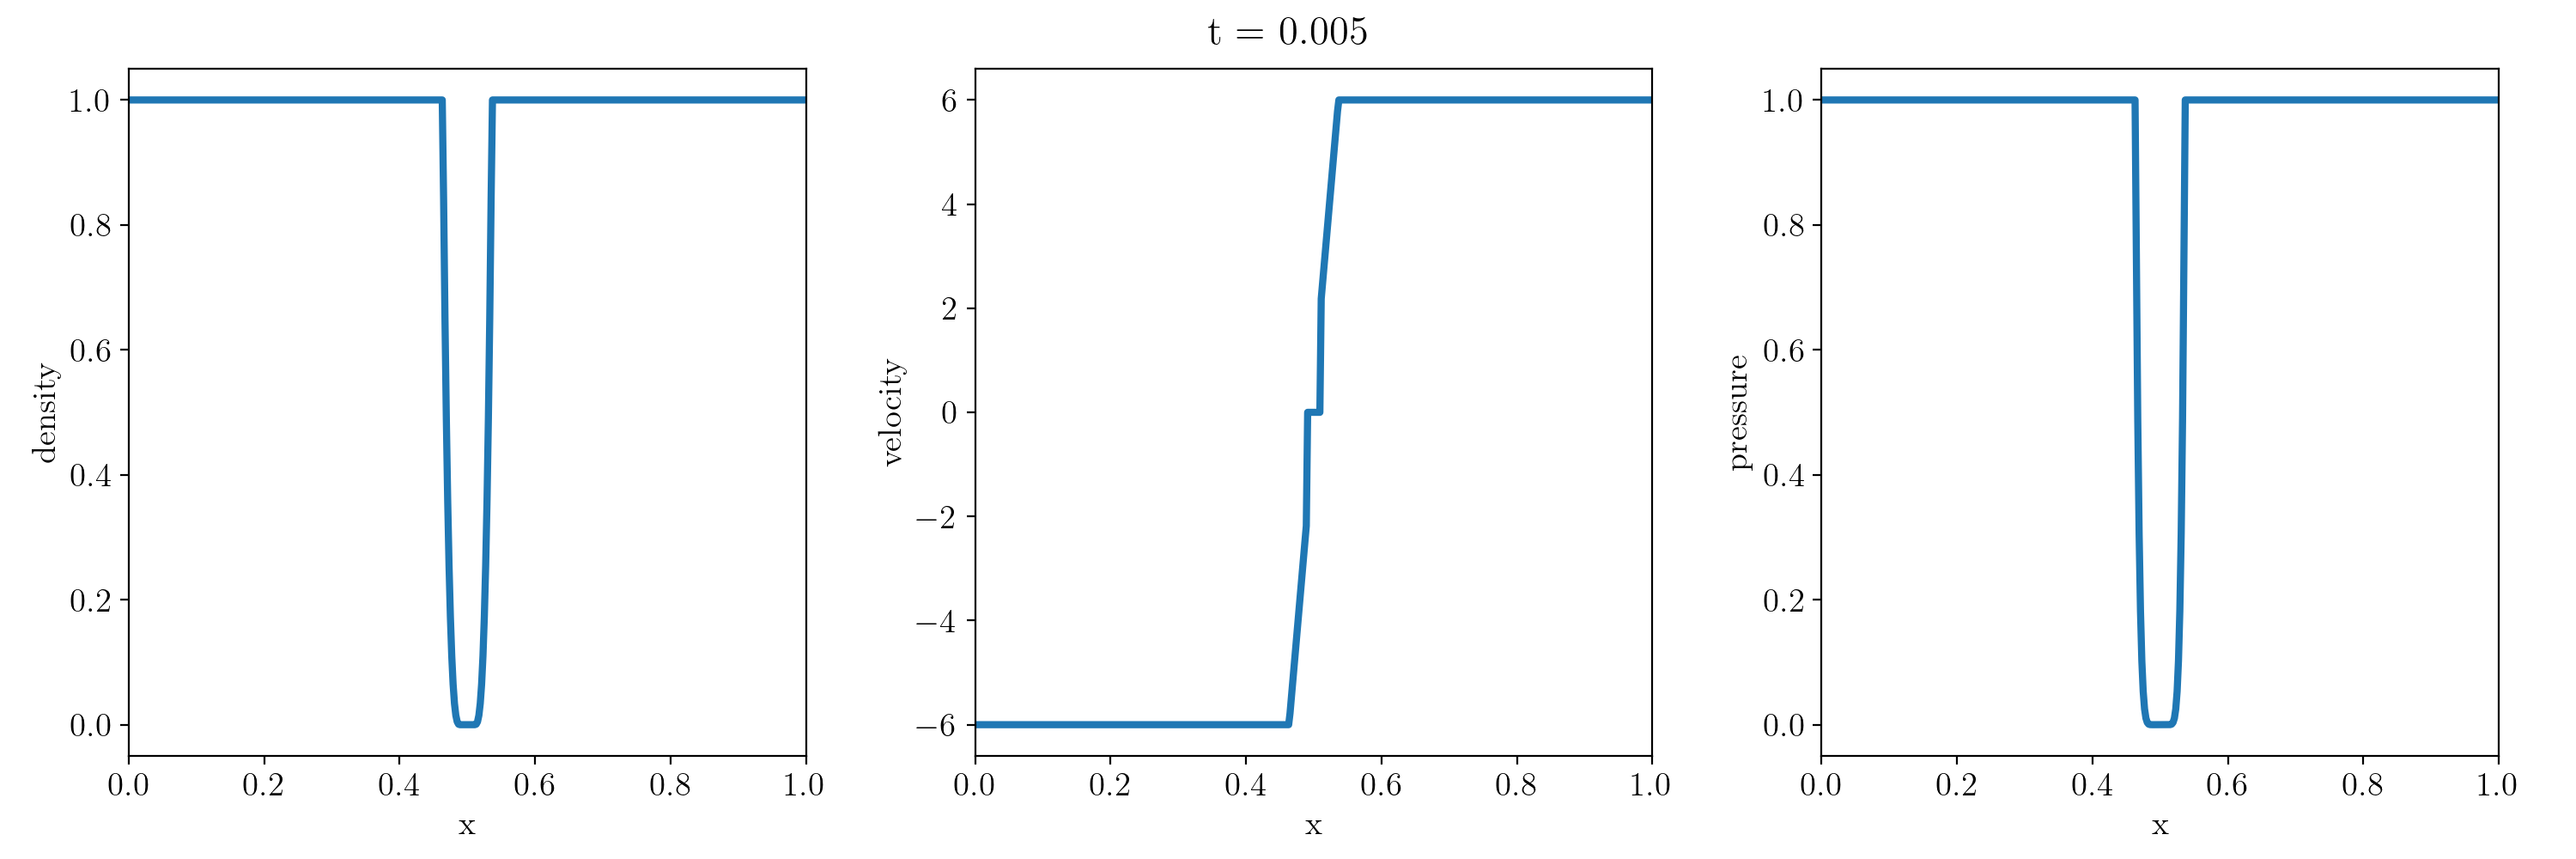
\includegraphics[width=\textwidth]{
./figures/FV/vacuum_generating_ICs/riemann-approximate-vacuum_generating-0.005.png} %
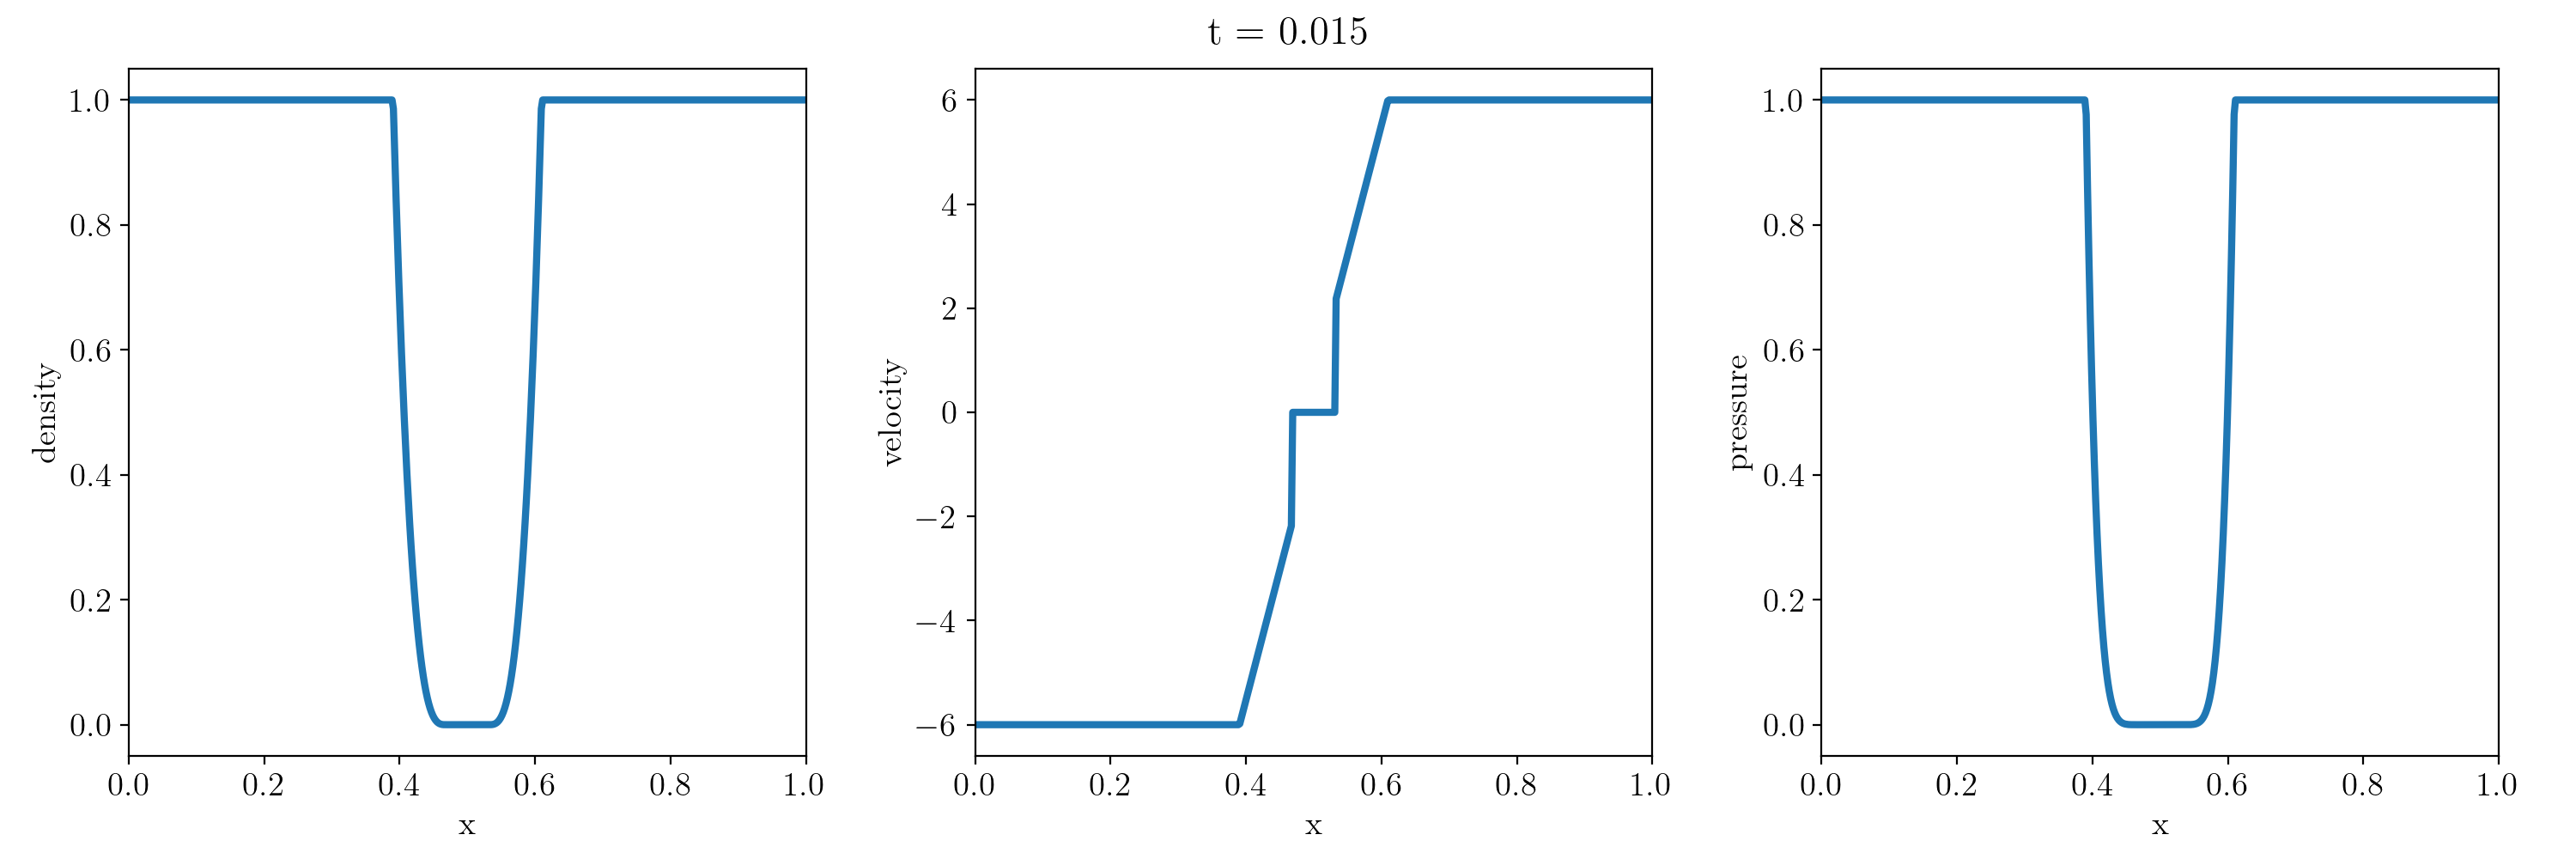
\includegraphics[width=\textwidth]{
./figures/FV/vacuum_generating_ICs/riemann-approximate-vacuum_generating-0.015.png} %
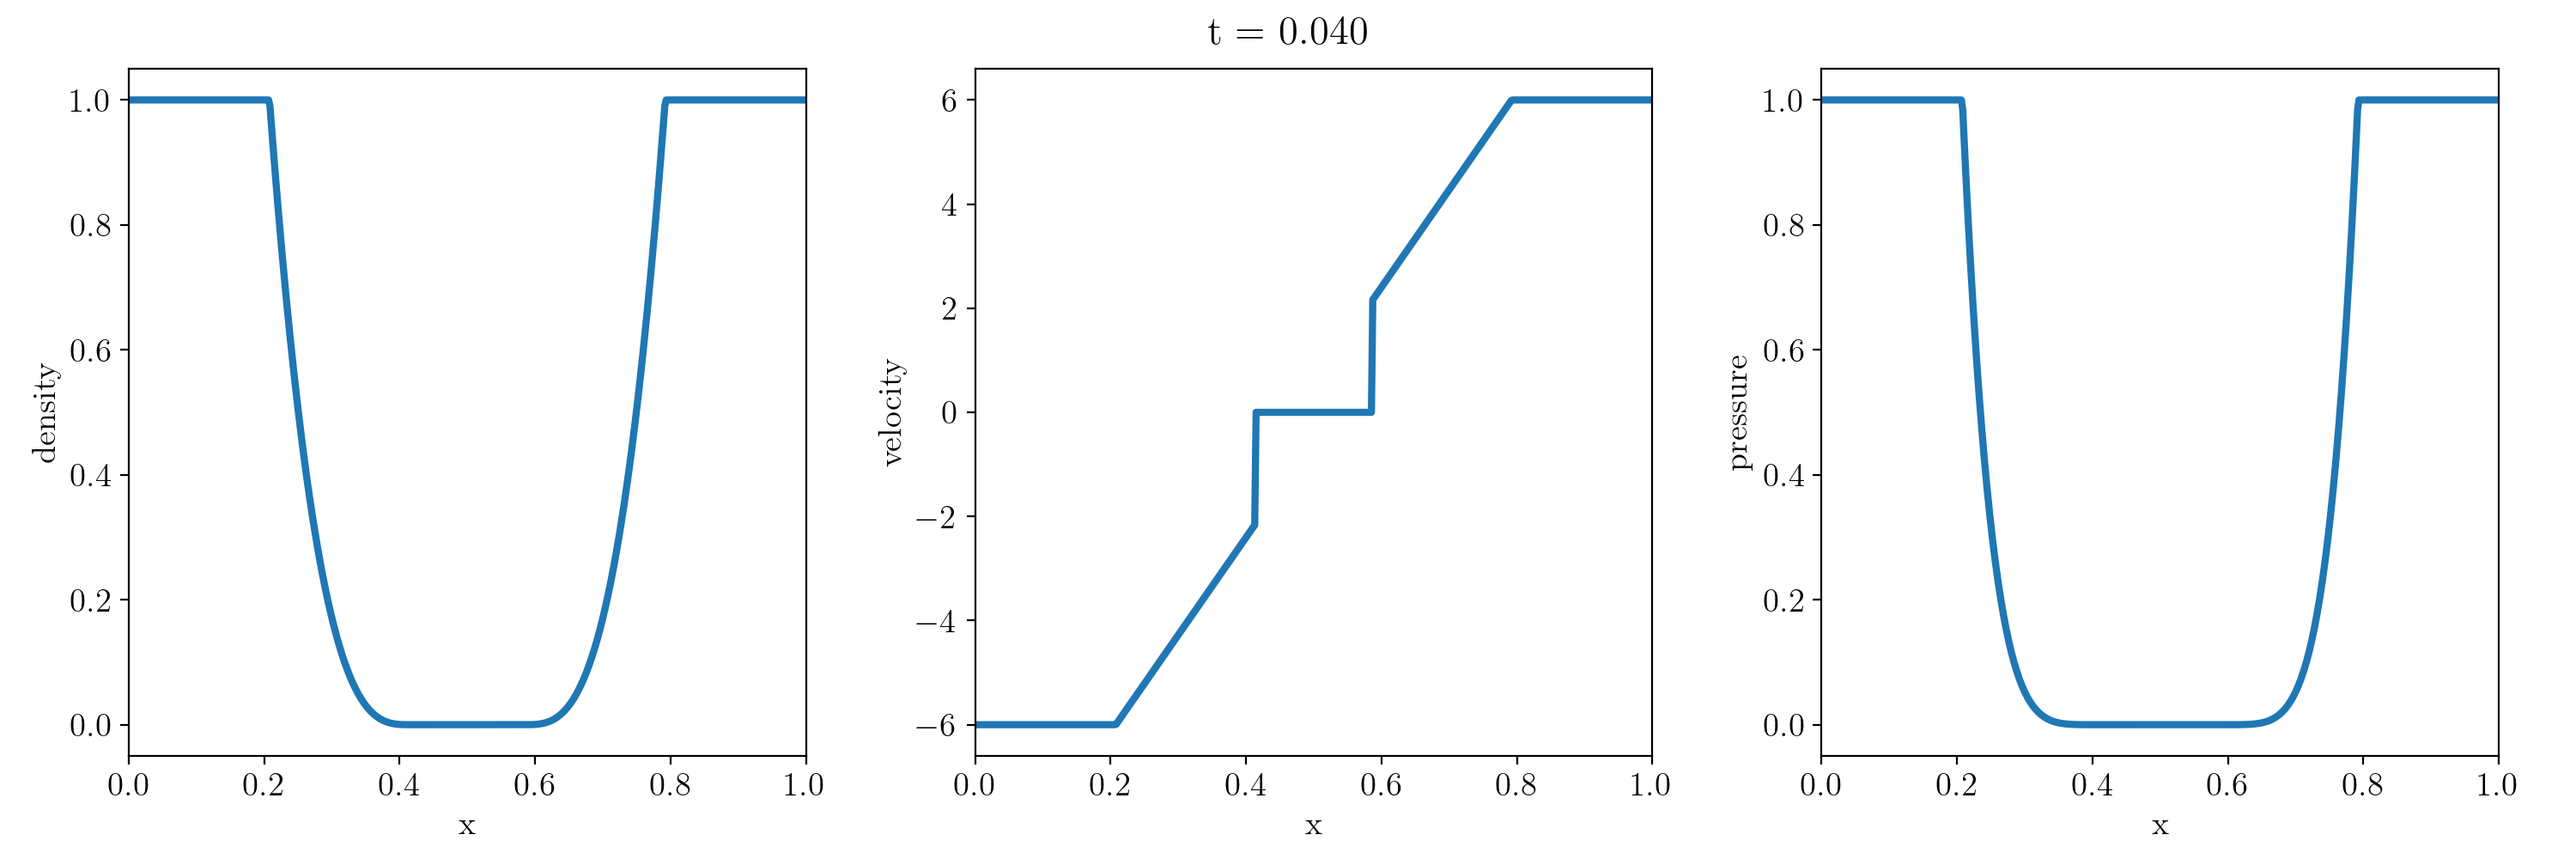
\includegraphics[width=\textwidth]{
./figures/FV/vacuum_generating_ICs/riemann-approximate-vacuum_generating-0.040.png} %
\caption[Riemann problem that generates a central vacuum]{
    Initial conditions and time evolution of a Riemann problem that generates vacuum in the central
    region.
    }%
    \label{fig:vacuum-generating}
\end{figure}













